\documentclass{beamer}

\usepackage[american,russian]{babel}

\usefonttheme{serif}

\setbeamertemplate{footline}[frame number]{}
\setbeamertemplate{navigation symbols}{}

\usecolortheme{default}
\setbeamercolor{block title}{bg=lily!20,fg=black}
\setbeamercolor{block body}{bg = blue!10, fg = black}
\setbeamertemplate{itemize item}[square]
\setbeamercolor{itemize item}{fg = cyan}
\setbeamercolor{enumerate item}{fg = cyan}

\usetheme{default}
\usepackage[justification=centering]{caption}

%\setbeamercolor{titlelike}{fg=cyan}
%Information to be included in the title page:

\title[About Beamer] %optional
{Оптический пробой сред}

%\subtitle{A short story}

\author[Arthur, Doe] % (optional, for multiple authors)
{Симанкович А.Л. \and Дедков Д.А. }

\institute[VFU] % (optional)
{
	Московский Физико-Технический Институт
}

\date[VLC 2023] % (optional)
%{Very Large Conference, April 2021}

%\logo{\includegraphics[height=1cm]{overleaf-logo}}

\begin{document}
	
	\frame{\titlepage}
	
	\begin{frame}
		\frametitle{Аннотация}
				
		% TODO: численные данные
		В работе рассмотрен эффект оптического пробоя воздуха фокусированным лазерным излучением. Приведено теоретическое описание образования пробоя в газах. Измерены спектры и осциллограммы пробойной искры для различных веществ.
		
		% TODO:
		Ключевые слова:
	\end{frame}


	\begin{frame}[plain,c]
		
		\begin{center}
			\huge \usebeamercolor[fg]{frametitle} Введение
		\end{center}
	
	\end{frame}
	
	
	\begin{frame}
		\frametitle{Статический пробой}

		\begin{figure}
			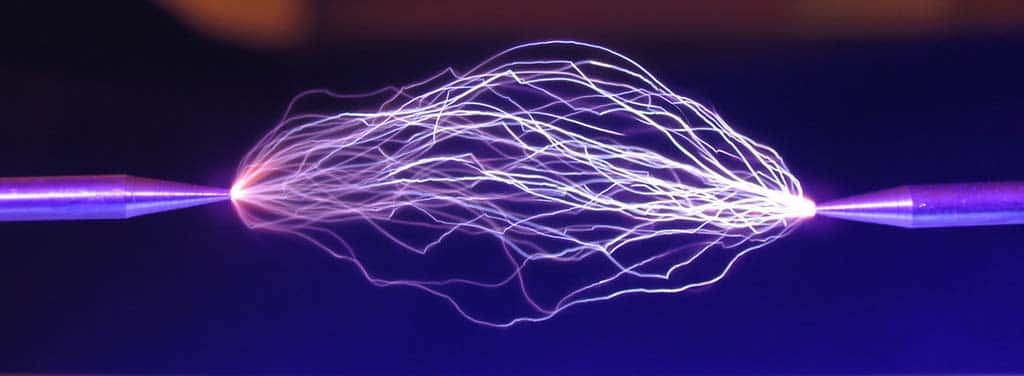
\includegraphics[width=0.8\linewidth]{res/const_discharge.jpg}
		\end{figure}
		
		\begin{columns}
			\column{0.6\linewidth}
			\begin{figure}
				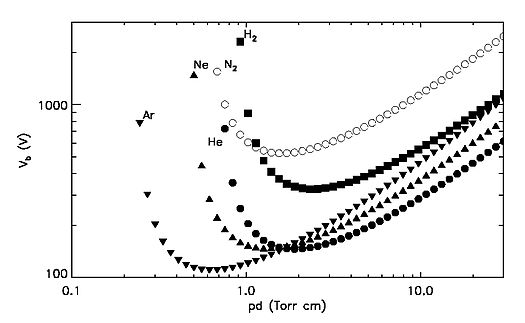
\includegraphics[width=\linewidth]{res/paschen.jpg}
			\end{figure}

			\column{0.5\linewidth}
			Пробой постоянным напряжением описывается кривыми Пашена.
		\end{columns}

%			Самый известный и хорошо изученный тип пробоя -- пробой постоянным напряжением. Его поведение в первом приближении описывается кривыми Пашена.
%			Заметим, что у кривой существует минимум.	
	\end{frame}

	\begin{frame}
		\frametitle{Пробой в переменных полях}
		
		\begin{columns}
			\column{0.15\linewidth}
			\begin{figure}
				\centering
				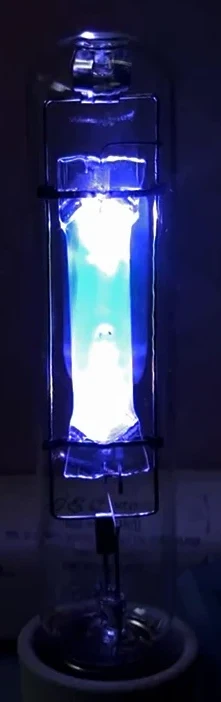
\includegraphics[width=1\linewidth]{res/hg_lamp.png}
				\caption*{Ртутная лампа}
			\end{figure}
			
			\column{0.7\linewidth}
			\begin{figure}
				\centering
				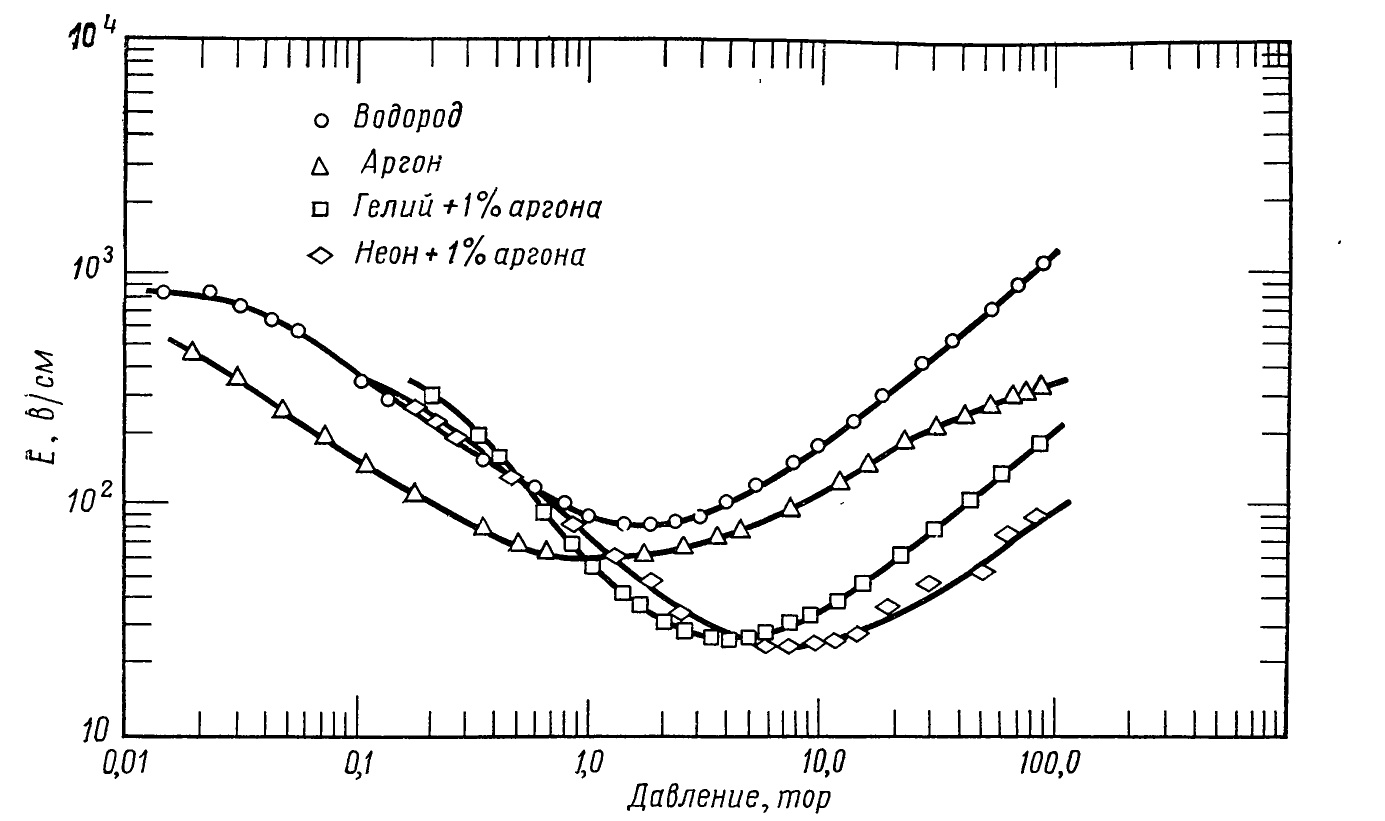
\includegraphics[width=1\linewidth]{res/microwave_discharge.png}
				\caption*{Зависимость пробойного поля от давления\\ ($f = 992$ МГц, диффузионная длина $0.631$ см)}
			\end{figure}
			
		\end{columns}		
		
		%TODO: ссылка на Microwave Breakdown in Gases by A. D. MacDONALD
		Переменное поле также индуцирует пробой.

%		Под действием переменного поля также возникает пробой. Его минимум для типичных параметров установки расположен в диапазоне давлений, близких к нормальному.
	\end{frame}

	\begin{frame}
		\frametitle{Оптический пробой}
		\begin{columns}
			\column{0.4\linewidth}
			\begin{figure}
				\centering
				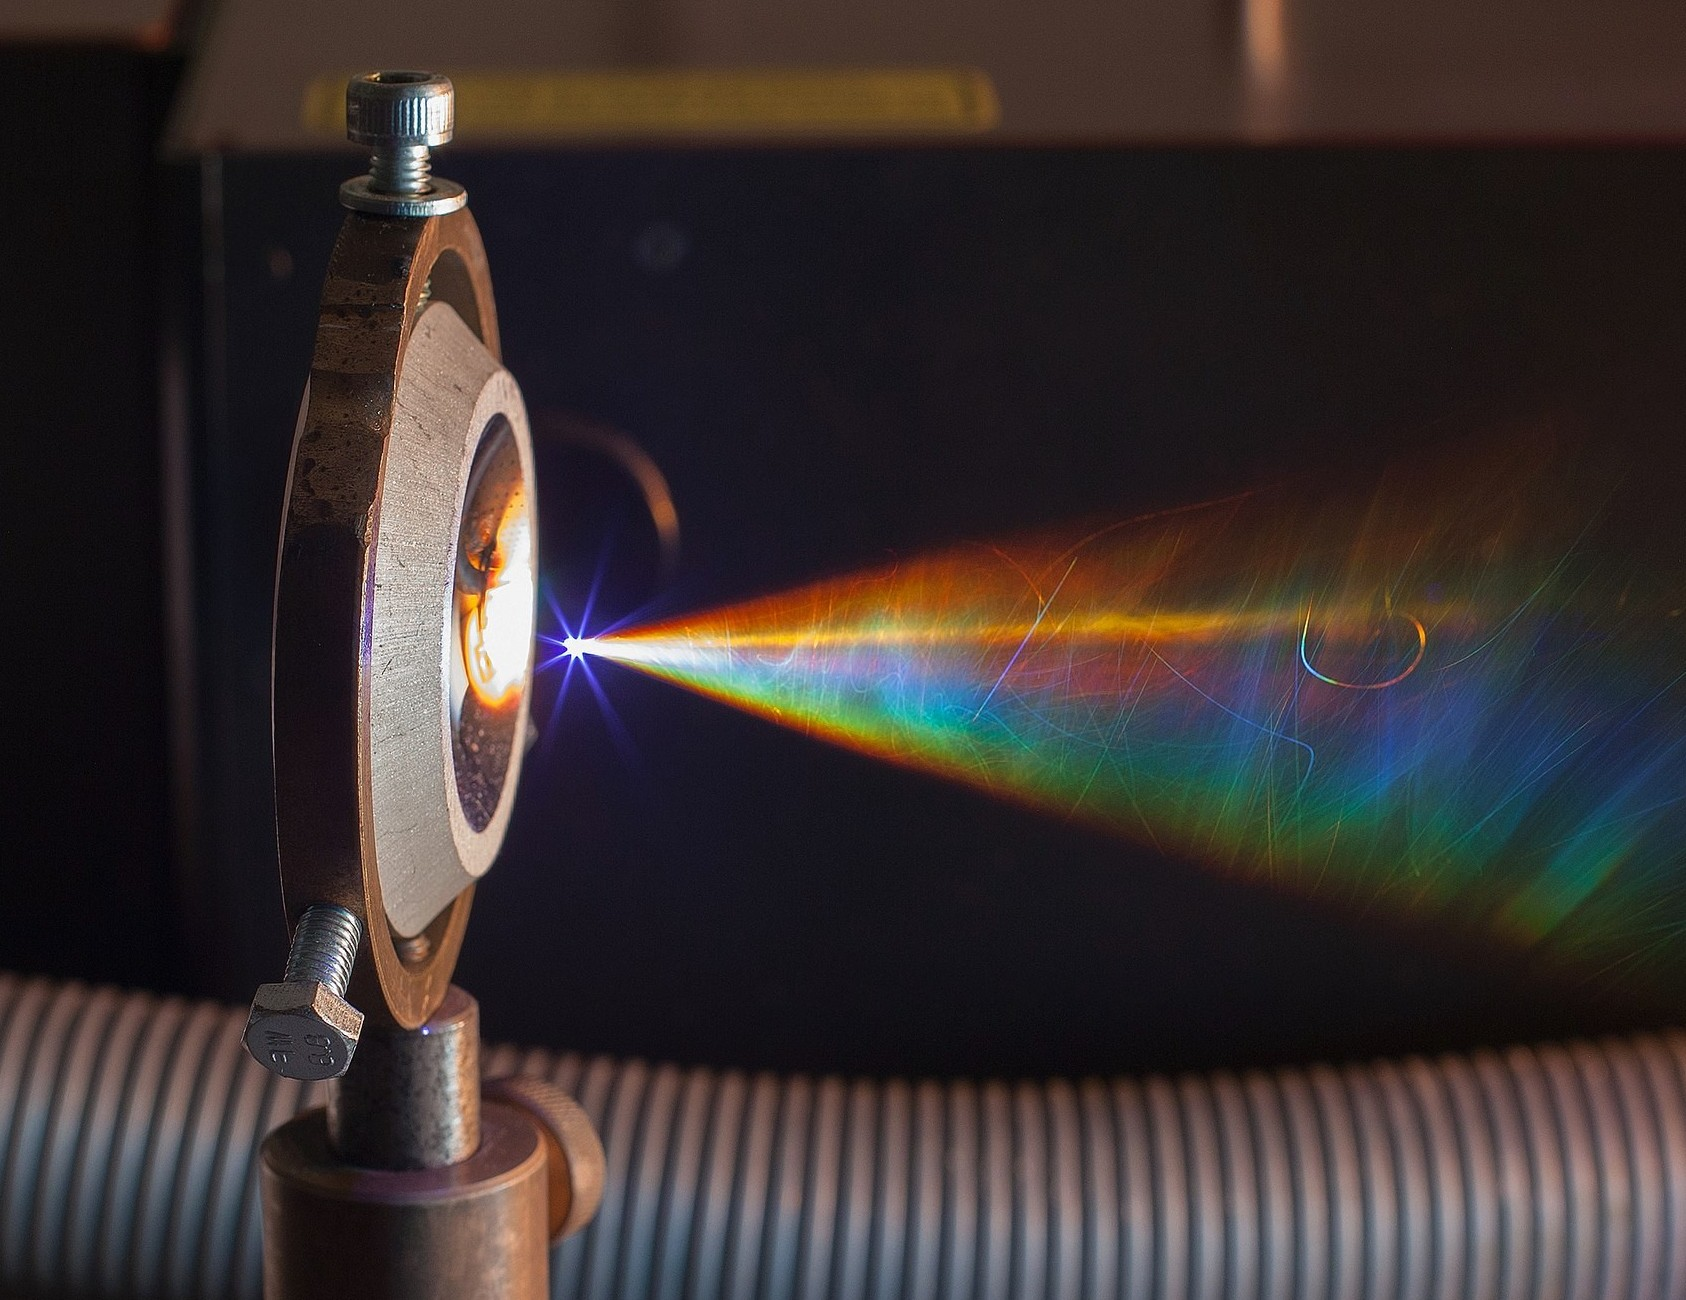
\includegraphics[width=1.05\linewidth]{res/new_femtosecond_laser_spark.jpg}
				\caption*{Пробой воздуха фемтосекундным лазером}
			\end{figure}
			
			\column{0.6\linewidth}
			\begin{figure}
				\centering
				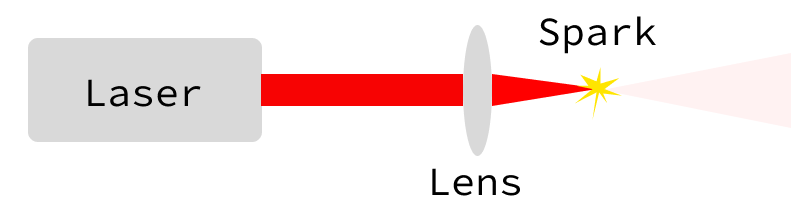
\includegraphics[width=1.0\linewidth]{res/scheme.png}
				\caption*{Принципиальная схема}
			\end{figure}
			
			
		\end{columns}
		%TODO: может не стоит вставлять картинку с непонятной радугой?
		\begin{itemize}
			\item Оптический пробой -- $E \approx 10^6 \div 10^7$ В/см 
			\item Постоянное и СВЧ поля -- $E \approx 3 \cdot 10^4$ В/см. 
		\end{itemize}
		Характерные параметры:
		$$ P \approx 30 \text{ МВт}, \quad d = 2 \cdot 10^{-2} \text{ см} $$
		$$ I \approx 10^5 \text{ МВт/см}^2, \quad E \approx 6 \cdot 10^6 \text{ В/см} $$

		%		В данной работе изучается пробой полем оптического диапазона. Характерные значения поля для пробоя газа $E \approx 10^6 \div 10^7$ В/см (для постоянного и СВЧ полей $E \approx 3 \cdot 10^4$ В/см). 

		%Такие величины полей достижимы только в фокусированном лазерном излучении: при пиковой мощности и диаметре фокуса $2 \cdot 10^{-2}$ см получаем $I \approx 10^5$ МВт/см$^2$ и поле $E = 6 \cdot 10^6$ В/см.
	
	\end{frame}

	\begin{frame}
		\frametitle{Применения лазерного пробоя}
	
		\begin{figure}
			\centering
			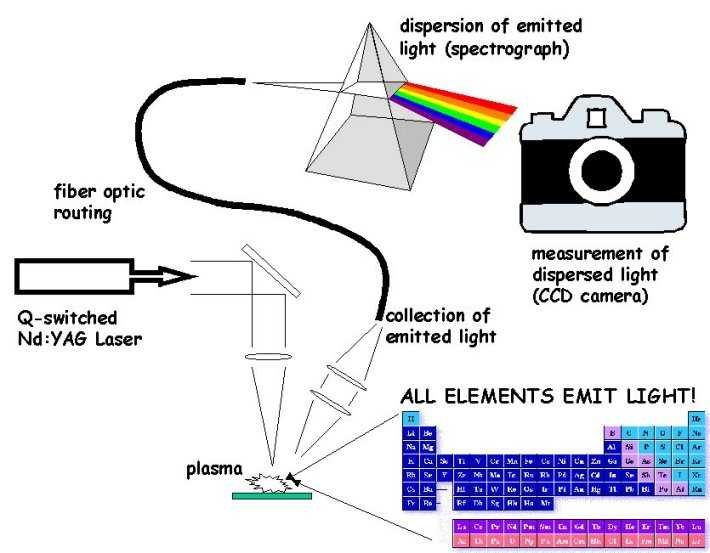
\includegraphics[width=0.5\linewidth]{res/libs.jpg}
			\caption*{Лазерно-искровая эмиссионная спектрометрия}
		\end{figure}
			
		\begin{itemize}
			\item Лазерно-искровая эмиссионная спектрометрия.
			\item Связан с термоядерным синтезом
			\item Развитие квантовой теории
		\end{itemize}

%		Лазерно-искровая эмиссионная спектрометрия --  основное прикладное применение лазерного пробоя.
%		
%		Явление лазерного пробоя тесно связано с задачами термоядерного синтеза.
%		
%		Изучение лазерного пробоя позволяет получить важные выводы для квантовой теории.
	\end{frame}
	
	\begin{frame}
		\frametitle{Стадии искры}
		\begin{figure}
			\centering
			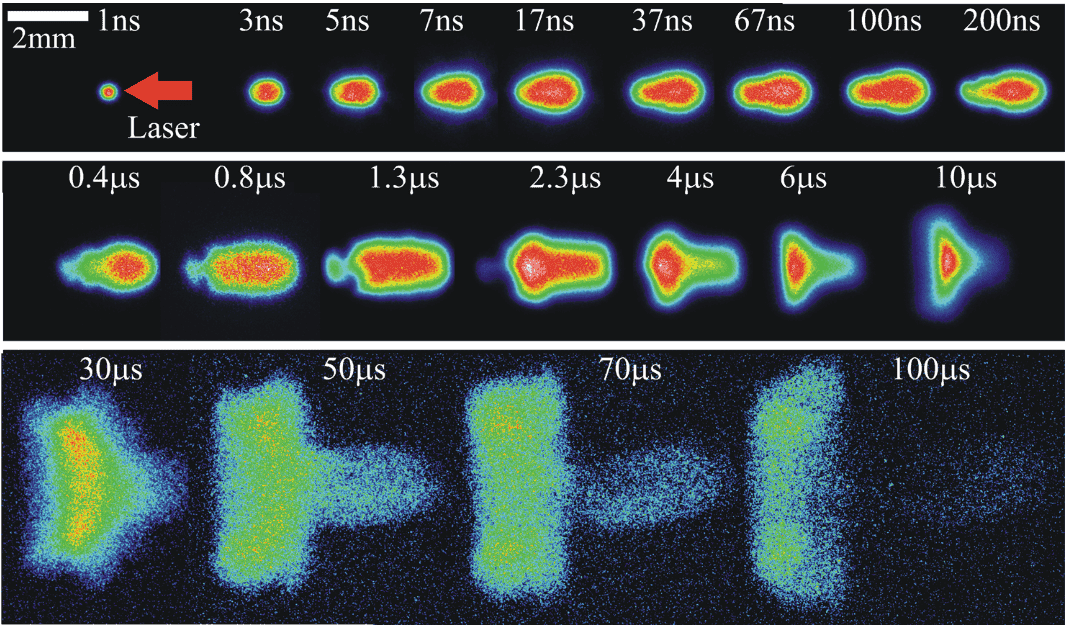
\includegraphics[width=0.8\linewidth]{res/spark_evolution.png}
			\caption*{Эволюция искры во времени}
		\end{figure}
		\vspace{-5pt}
		Три стадии лазерной искры:
		\begin{itemize}
			\item Пробой: ионизация и появление начальной плазмы.
			\item Взаимодействие плазмы с лазерным импульсом, движение плазменного фронта.
			\item Распространение ударной волны, свечение.
		\end{itemize}
	\end{frame}
	
	
	\begin{frame}[plain,c]
		
		\begin{center}
			\huge \usebeamercolor[fg]{frametitle} Теория
		\end{center}
		
	\end{frame}
	
		\begin{frame}
		\frametitle{Начало пробоя -- ионизация излучением}
		\vspace{-5pt}
		Два механизма вырывания электрона из атома излучением:
		% TODO: А может в постоянном поле быть "просто достаточное поле", чтобы быть сильнее притяжения электрона к ядру? Это тоже туннельный эффект?
		\begin{columns}
			\column{0.5\linewidth}
			\begin{figure}
				\centering
				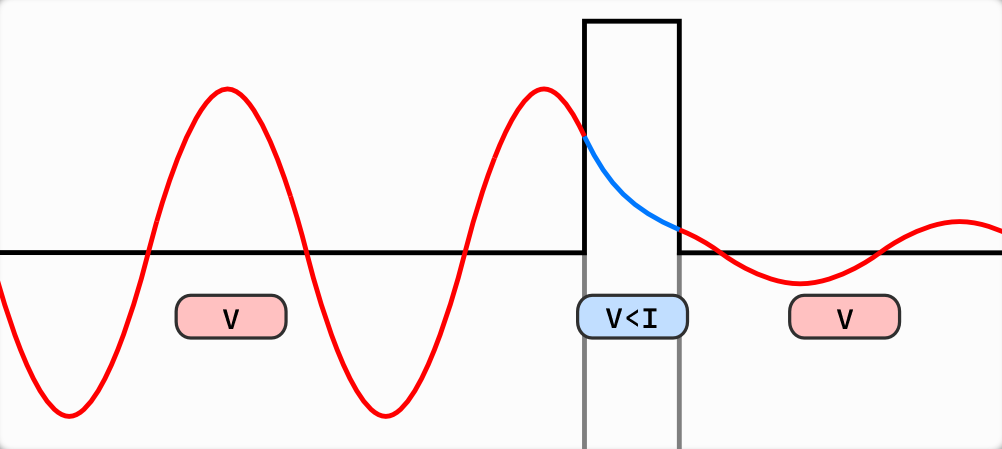
\includegraphics[width=\linewidth]{res/tunneling.png}
				\caption*{Туннельный эффект}
			\end{figure}
			\vspace{-10pt}
			\footnotesize
			\begin{itemize}
				\setlength\itemsep{-2pt}
				\item $E$ -- поле световой волны.
				\item $I$ -- энергия ионизации.
				\item $\Delta \sim \frac{I}{eE}$ -- ширина потенциального барьера.
				\item $v \sim \sqrt{I/m}$ -- скорость электрона.
				\item $\tau \sim \Delta / v \sim \frac{\sqrt{Im}}{eE}$ -- время пролета барьера.
			\end{itemize}
			$$\omega \tau \ll 1 \text{ -- условие статичности поля.}$$
			
			\column{0.5\linewidth}
			\begin{figure}
				\centering
				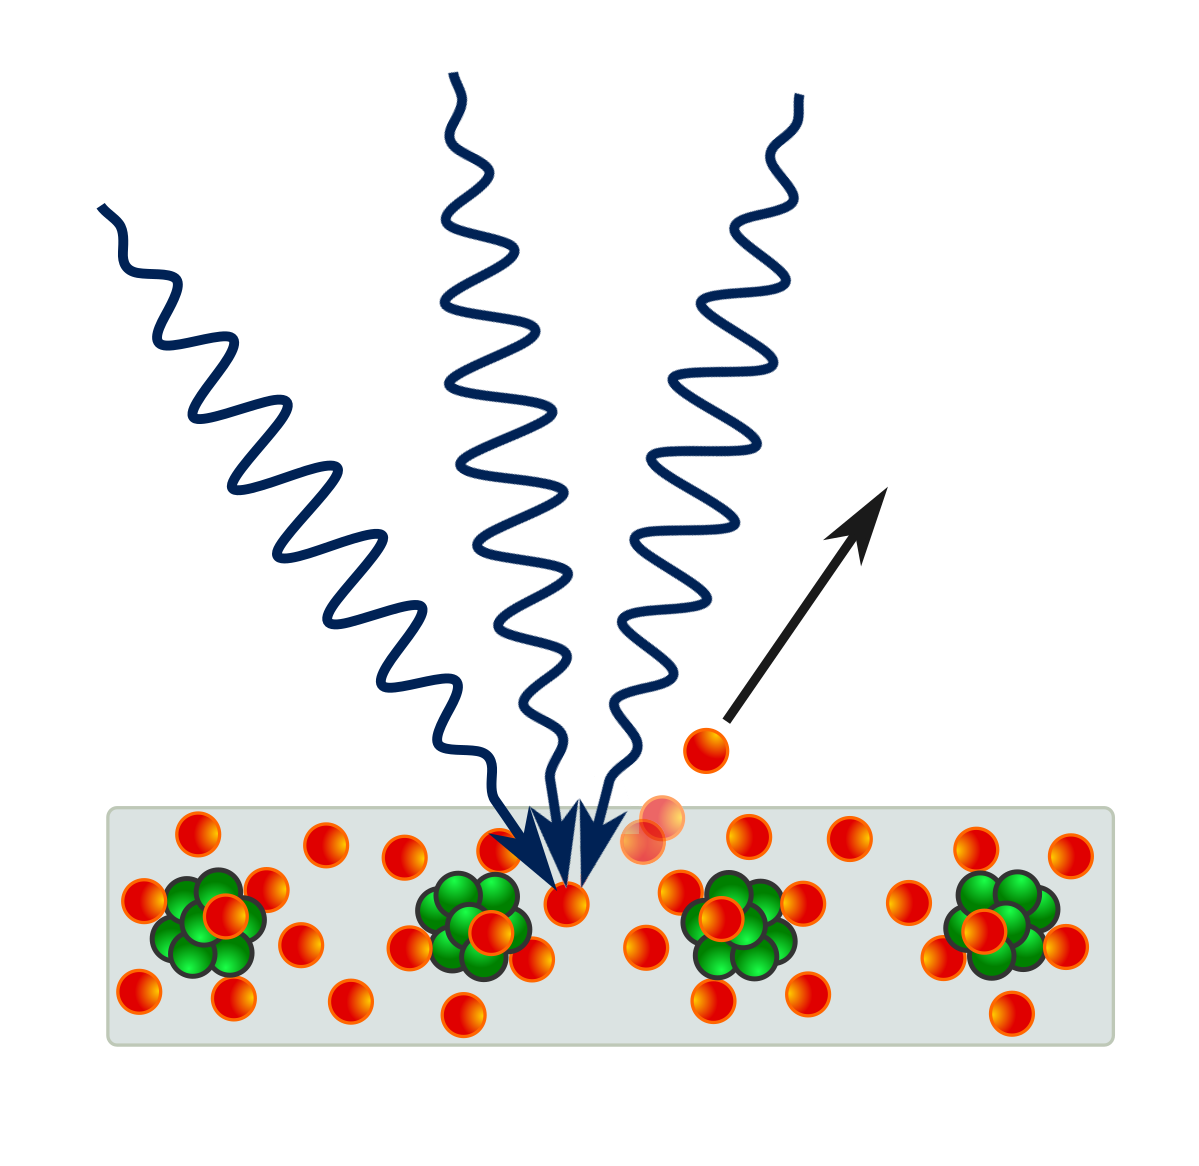
\includegraphics[width=0.7\linewidth]{res/multiphoton.png}
				\caption*{Многоквантовый фотоэффект}
			\end{figure}
			\footnotesize
			$\omega \tau \gg 1$ -- условие получения достаточного числа квантов за колебание.
		\end{columns}
		\vspace{10pt}
		Оценка для пробоя на оптических частотах дает $\omega \tau \gg 1$.
		%Для вырывания электрона из атома есть два механизма: туннельный эффект (например, в статическом электрическом поле) и многоквантовый фотоэффект.
		%Ширина потенциального барьера под действием поля $E$ составляет $\Delta \sim \frac{I}{eE}$. Скорость электрона $v \sim \sqrt{I/m}$. Тогда время пролета барьера $\tau \sim \Delta / v \sim \frac{\sqrt{Im}}{eE}$. Туннелирование может происходить если поле остается 'стационарным' во время пролета барьера: $\omega \tau \ll 1$. Для многоквантовости требуется обратное неравенство: $\omega \tau \gg 1$. Для типичных значений лазерного излучения характерно $\omega \tau \gg 1$.
		
	\end{frame}
	
	\begin{frame}
		\frametitle{Вероятность многоквантового фотоэффекта}
		\begin{itemize}
			\setlength\itemsep{-2pt}
			\item $w$ -- вероятность многоквантового фотоэффекта
			\item $n$ -- количество поглощаемых фотонов
			\item $S$ -- интенсивность
		\end{itemize}
		
		$w \sim S \sim E^2$ -- вероятность пропорциональна интенсивности.
		
		$w \sim \frac{1}{I}$ -- чем выше порог ионизации, тем ниже вероятность.
		
		$w \sim \frac{1}{\omega}$ -- чем ниже частота, тем больше время, за которое электрон может поглотить нужную энергию.

		$w \sim (...)^n$ -- $n$-кратное поглощение.
		
		$$ w \sim \left(\frac{E^2}{\omega I}\right)^n$$
		
		Результат полученный Л.В.Келдышем в рамках квантовой механики:
		\begin{equation}
			w = B \omega n^{3/2} \left(\frac{\overline{e} e^2 E^2}{8m \omega^2 I}\right)^n
		\end{equation}
		%Вероятность многоквантового фотоэффекта $w$ с поглощением $n$ фотонов пропорциональна $n$-ой степени потока квантов $w \sim F^n$, то есть $w \sim E^{2n}$.
		%$w \sim \frac{1}{I^n}$ -- чем выше порог ионизации, тем ниже вероятность.
		%$w \sim \frac{1}{\omega^n}$ -- чем ниже частота поля, тем больше характерное время изменения поля, за которое электрон может поглотить нужную энергию.
		%$$ w \sim \left(\frac{E^2}{\omega I}\right)^n$$
		%Точный расчет был произведен Л.В.Келдышем с использованием квантовой механики, его результат для фотоэффекта можно аппроксимировать следующей формулой:
		%$$ w = B \omega n^{3/2} \left(\frac{\overline{e} \pi e^2}{mc} \frac{\hbar E}{\omega I}\right)^n,$$
		%где $\omega$ -- частота поля, $B$ -- константа около 1, $$\overline{e}$ -- математическая константа, $e$ -- заряд электрона, $\hbar$ -- константа Планка.
		
		%TODO: Райзер, с 15, дописать численную оценку
		%Получить формулу как-то просто не получается(
	\end{frame}
	
	\begin{frame}
		\frametitle{Оценка порогового поля}
		
		За время $t_1 \approx 40 \text{ нс}$ в пятне радиусом $r$ должно появиться $N = 10^{13}$ электронов:
		$$N = \frac{4}{3} \pi r^3 N_a t_1 w$$
		\begin{center}
			\boxed{E = \sqrt{\frac{8m\omega^2 I}{\overline{e} e^2}} \left[\frac{w}{\omega n^{3/2}}\right]^{1/2n}}
		\end{center}
	
		Для аргона:
		$$ E = 1.12 \cdot 10^8 \text{ В/см -- оценка}$$
		$$ E = 2.69 \cdot 10^6 \text{ В/см -- эксперимент}$$
		
	\end{frame}
	
	\begin{frame}
		\frametitle{Развитие пробоя -- электронная лавина}
		
		\begin{columns}
			\column{0.5\linewidth}
			\begin{figure}
				\centering
				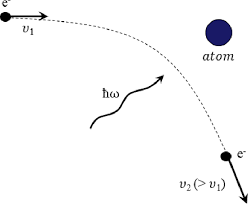
\includegraphics[width=0.7\linewidth]{res/inverse_bremsstrahlung.png}
				\caption*{Процесс, обратный тормозному излучению}
			\end{figure}
			\column{0.5\linewidth}
			\begin{itemize}
				\item Классика: в переменном поле энергия колебаний при столкновениях переходит в тепло.
				\item Квантовая: электрон поглощает фотоны при столкновениях.
			\end{itemize}
%			В осциллирующем поле, при колебании электронов, в среднем энергия электронов при столкновениях переходит в тепло.
%			По квантовой теории электрон поглощает фотоны при столкновениях с атомами.
		\end{columns}
		\begin{columns}
			\column{0.5\linewidth}
			\begin{figure}
				\centering
				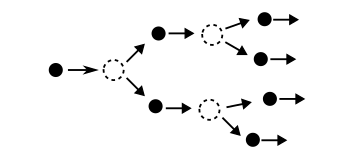
\includegraphics[width=0.8\linewidth]{res/electron_avalanche.png}
				\caption*{Электронная лавина}
			\end{figure}
		
			\column{0.5\linewidth}
			Формируется электронная лавина.
			
		\end{columns}		
		
		
		% 1.
		% Под действием постоянного внешнего электрического поля свободные электроны ускоряются, при столкновении с атомом рассеивая эту энергию в тепло. В осциллирующем поле, при колебании электронов, в среднем энергия электронов при столкновениях тоже переходит в тепло (что будет показано далее).
		% Для оптического диапазона разумнее использовать квантовую теорию. При столкновениях с атомами электрон поглощает фотоны, приобретая энергию. Этот процесс обратен тормозному испусканию квантов при рассеянии.
		% Таким образом, в области поля средняя скорость электронов увеличивается. Эти электроны набирают достаточную энергию, чтобы ионизировать атомы. Новые электроны добавляются к свободным, увеличивая скорость ионизации. Формируется электронная лавина.
		
	\end{frame}

	\begin{frame}
		\frametitle{Развитие пробоя -- многоквантовый фотоэффект}
		
		\begin{columns}
			\column{0.5\linewidth}
			\begin{figure}
				\centering
				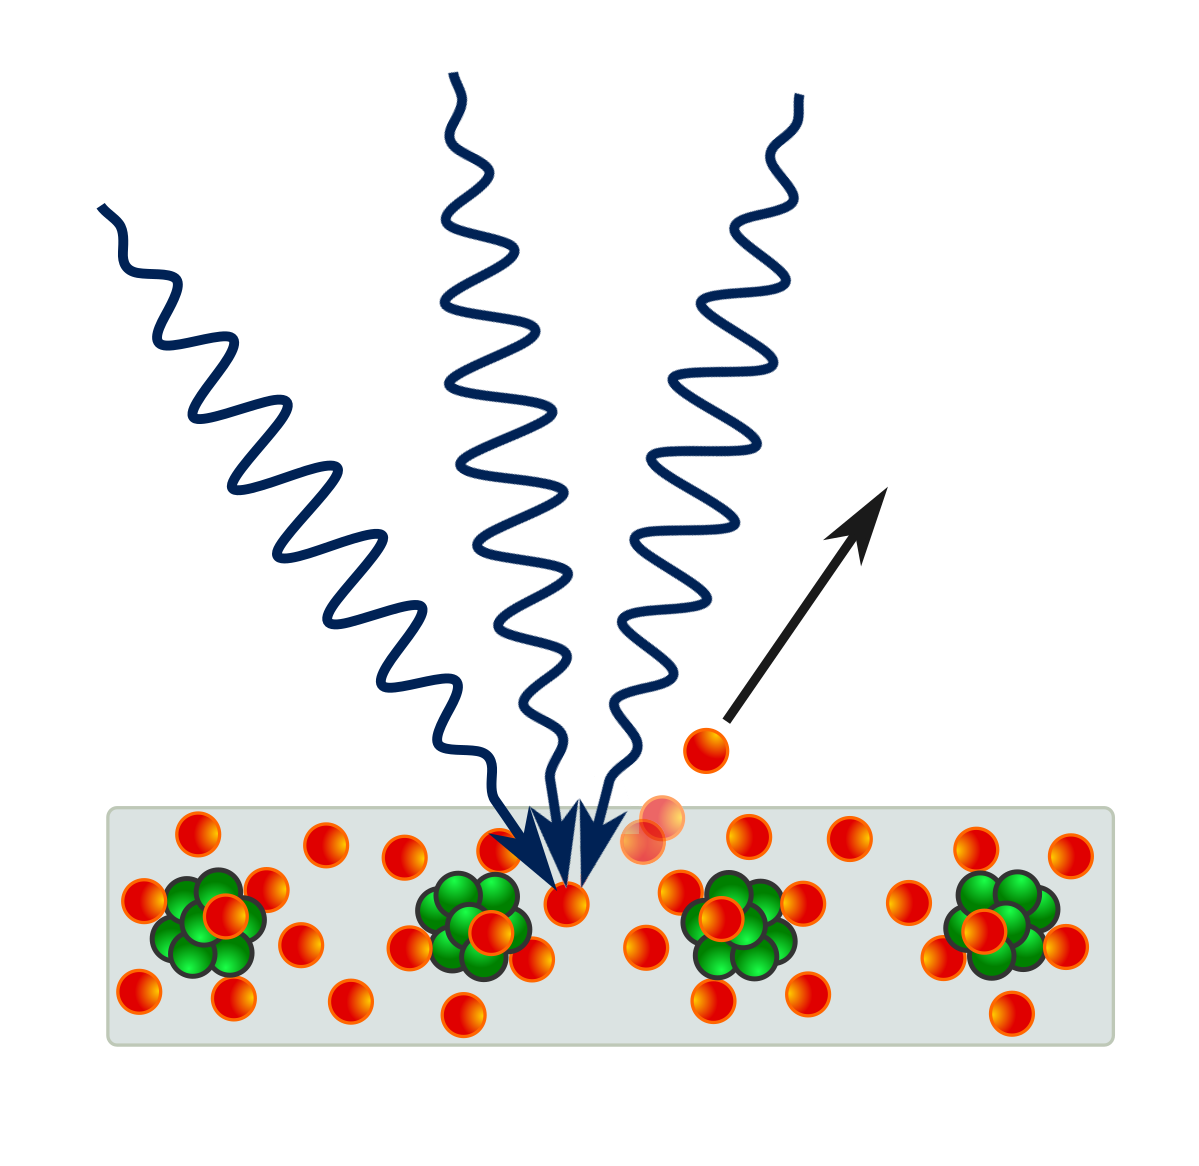
\includegraphics[width=0.9\linewidth]{res/multiphoton.png}
				\caption*{Многоквантовый фотоэффект}
			\end{figure}
		
			\column{0.5\linewidth}
			Электрон поглощает несколько фотонов одновременно. 
			$$n \cdot h\nu \sim n \cdot 2 \text{ эВ} > I \sim 10 \div 20 \text{ эВ}$$
		\end{columns}
	
		Развитие пробоя:
		\begin{itemize}
			\item $p \geqslant 1\text{ атм}$ -- электронная лавина.
			\item $p \ll 1\text{ атм}$ -- многоквантовый фотоэффект.
		\end{itemize}
%		Для газов при давлениях порядка атмосферного и выше -- электронная лавина.
%		Для разреженных -- многоквантовый фотоэффект.
		% 2.
		% Вторым механизмом является многоквантовый фотоэффект. Электрон может оторваться от атома вследствие одновременного поглощения сразу нескольких фотонов. Одноквантовый эффект невозможен, так как энергия ионизации ()$I \sim 10\div20$ эВ) на порядок выше энергии фотонов видимого диапазона ($ h\nu = \sim 2$ эВ).
		% Для газов при атмосферных давлениях и выше характерен первый механизм.
	\end{frame}
	
	\begin{frame}
		\frametitle{Нарастание энергии -- классический случай}
		%TODO: Райзер, с 19-22 (вывод довольно простой)
		
		%KEKW: Классическая теория не описывает оптический диапазон: $h\nu >> \varepsilon_{\text{кол}}$.
		
		%KEKWKEKW: А нет, описывает: $ h \nu >> \varepsilon_{\text{кол}}$, но $h\nu << \varepsilon$, а это новое условие применения классики (Райзер, с 40, 43)
		
		\begin{columns}
			\column{0.5\linewidth}
			\begin{figure}
				\centering
				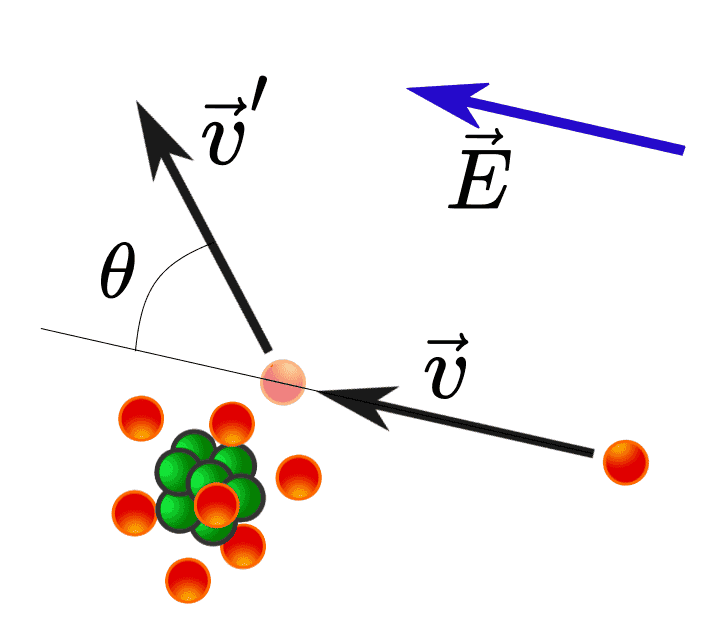
\includegraphics[width=0.8\linewidth]{res/collision.png}
				\caption*{Рассеяние электрона}
			\end{figure}
			
			\column{0.5\linewidth}
			Изолированный электрон не забирает энергию у поля. Получать энергию можно только за счет столкновений.
			$$ \varepsilon_{\text{кол}} = e^2 E_0^2/4m\omega^2 \sim 0.01 \text{ эВ}$$
			$$ \varepsilon \sim 10 \text{ эВ} \text{ -- энергия электрона}$$
			\begin{center}
				\boxed{\varepsilon \gg \varepsilon_{\text{кол}} \gg h \nu}
			\end{center}
		\end{columns}
		
		Уравнение движения с 'силой трения':
		$$ m \dot{v} = - m v \nu_m - e E \qquad E = E_0 \exp(-i \omega t)$$
		$\nu_m = \nu_c (\overline{1 - \cos \theta})$ -- эффективная частота столкновений.
		
		Работа, совершаемая полем над электроном:
		\begin{equation}
			\boxed{d\varepsilon/dt = \frac{e^2 E^2 \nu_m}{m (\omega^2 + \nu_m^2)}
			\label{eq:energy_growth}}
		\end{equation}

%		Изолированный электрон, не испытывающий столкновений с атомами, не забирает энергию у поля, получив ее лишь единожды при появлении поля. Получать энергию можно только за счет столкновений.
%		
%		Подразумевается, что электрон успевает набрать полную энергию колебаний $\varepsilon_{\text{кол}} = e^2 E_0^2/4m\omega^2$ за время между столкновениями.
%
%		Для СВЧ $\hbar \omega \ll \varepsilon_{\text{кол}}$, то есть энергия колебаний составляет много квантов и процесс описывается классически.
%		
%		Распределяя изменение импульса от удара на промежуток времени между столкновениями мы можем заменить резкие изменения на эквивалентную силу трения, которая рассеивает импульс.
%		
%		$$ m \dot{v} = - m v \nu_m - e E \qquad E = E_0 exp(-i \omega t)$$
%		$\nu_m = \nu_c (1 - \overline{1 - \cos \theta})$ -- частота столкновений с учетом угла рассеяния.
%		Решением уравнения является:
%		$$ v = - i e E/m (\omega + i \nu_m)$$
%		
%		Работа, совершаемая полем над электроном
%		\begin{equation}
%			d\varepsilon/dt = \frac{e^2 E^2 \nu_m}{m (\omega^2 + \nu_m^2)}
%			\label{eq:energy_growth}
%		\end{equation}
%		Среднее приращение за столкновение
%		$$ \Delta \varepsilon = 2 \varepsilon_{\text{кол}} \frac{\omega^2}{\omega^2 + \nu_m^2}$$
%		
%		С учетом передачи энергии атому в упругом столкновении
%		$$ d\varepsilon/dt = \nu_m \left[\frac{e^2 E^2}{m (\omega^2 + \nu_m^2)} - \frac{2m}{M}\varepsilon\right]$$
		
	\end{frame}

	\begin{frame}
		\frametitle{Нарастание энергии -- квантовый подход}
		
		\begin{columns}
			\column{0.5\linewidth}
			\begin{figure}
				\centering
				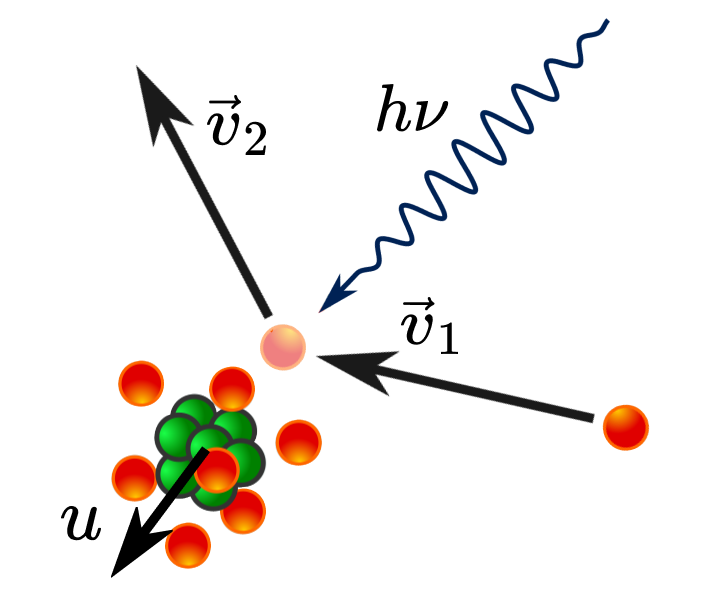
\includegraphics[width=0.8\linewidth]{res/collision_with_recoil.png}
				\caption*{Поглощение фотона}
			\end{figure}
			
			\column{0.5\linewidth}
			Энергия фотонов во много раз превосходит энергию колебаний:
			$$  h\nu = 1.8 \text{ эВ} \gg\varepsilon_{\text{кол}} \approx 2.3\cdot 10^{-2} \text{ эВ} $$
			\footnotesize
			\emph{(для рубинового лазера, $\omega = 2.7 \cdot 10^{15} \text{ Гц}, E \approx 10^7 \text{ В/см}$)}.
		\end{columns}
		
		Квантовая механика показывает, что классическая формула является применимой в условиях: 
		\begin{center}
			\boxed{\varepsilon \gg h\nu \gg \varepsilon_{\text{кол}}}
		\end{center}

		\footnotesize
		\emph{Энергии электрона $\varepsilon \approx 10 \text{ эВ}$ позволяют применять данную формулу}.
		
		
		
%		Отметим, что для фотонов не выполняется требование $\varepsilon_{\text{кол}} \approx 2.3\cdot 10^{-2} \text{ эВ} \ll h\nu = 1.8 \text{ эВ}$ (значения для рубинового лазера $\omega = 2.7 \cdot 10^{15} \text{ Гц}, E \approx 10^7 \text{ В/см}$).
%		t_1^{-1} ln( N_1 / N_0)
%		Как же быть?
%		
%		Столкновения все также остаются важны, так как изолированный электрон не может поглощать фотоны -- это противоречит ЗСИ.
%		
%		Поглощение и излучение фотонов электронами при столкновениях -- обратные друг другу процессы с близкими вероятностями, но поглощение происходит немного чаще.
%		
%		Более тщательные выкладки с использованием квантовой механики показывают, что классическая формула является применимой в условиях $\varepsilon \gg h\nu$.
%		Значения $\varepsilon \approx 10 \text{ эВ}$ позволяют применять данную формулу для оценок.
	\end{frame}
	
	\begin{frame}
		\frametitle{Потери энергии электронов}
		
		Существует два рода потерь: упругие и неупругие.
		
		\begin{columns}[t]
			\column{0.33\linewidth}
			\begin{figure}
				\centering
				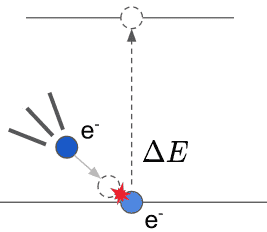
\includegraphics[width=0.8\linewidth]{res/excitation.png}
				\caption*{Возбуждение столкновением}
			
				Работают при энергиях $2/3I \div 3/4I$ (инертные газы).
			\end{figure}
		
			\column{0.33\linewidth}
			\vspace{10pt}
			\begin{figure}
				\centering
				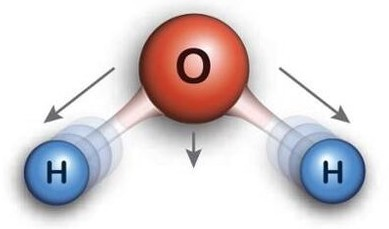
\includegraphics[width=1.0\linewidth]{res/vibrations.jpg}
				\caption*{Колебательные степени свободы}
				
				Работают для молекулярных газов даже при малых энергиях электронов.
			\end{figure}
			
			\column{0.33\linewidth}
			\begin{figure}
				\centering
				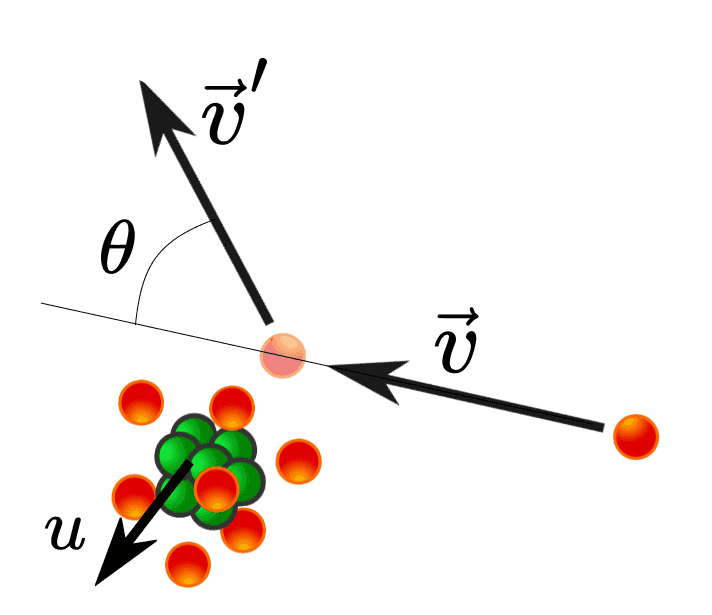
\includegraphics[width=0.8\linewidth]{res/recoil_loss.png}
				\caption*{Отдача энергии при столкновении}
				
				Работают при любых столкновениях с атомами.
			\end{figure}
			
		\end{columns}
		
%		Существует два рода потерь: упругие и неупругие.
%		
%		Упругие: отдача части энергии атому при соударении. Роль тем больше, чем легче газ. Работают при всех значениях энергии электрона.
%		
%		Неупругие: колебательные состояния молекулярных газов.
%		Неупругие: Возбуждение атомов. Работают при энергии $2/3I \div 3/4I$ (инертные газы).
%		
%		Для лавины (статика, СВЧ) возбуждение атомов губительно, поскольку на зарождении лавины электронов мало и шансов для попадания энергичного (хоть и не достаточно для ионизации невозбужденного) электрона с возбужденным мала.
%		
%		Для оптических частот для возбужденных атомов есть повышение вероятности многоквантового фотоэффекта. Но не на всех частотах это действительно улучшает показатели.
%		
	\end{frame}
	
	\begin{frame}
		\frametitle{Потери электронов}
		
		\begin{figure}
			\centering
			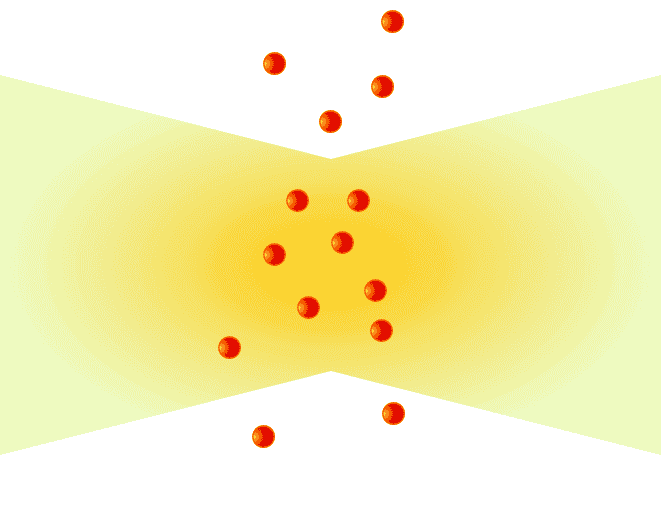
\includegraphics[width=0.5\linewidth]{res/diffusion.png}
			\caption*{Диффузия электронов}
		\end{figure}
		
		Основной механизм потерь -- диффузия из области фокусного пятна.
				
	\end{frame}

	\begin{frame}
		\frametitle{Критерий пробоя}
		Число электронов:
		$$ N_e = N_0 e^{\left[(\nu_i - \nu_d) t\right]} = N_0 e^{(t/\theta)},$$
		$\theta = (\nu_i - \nu_d)^{-1}$ -- постоянная времени лавины,\\
		$\nu_i$ -- частота ионизации атомов электронами,\\
		$\nu_d$ -- частота диффузионных уходов.

		За время импульса $t_1 \approx 30 \div 50$ нс должно появиться $N_1 \approx 10^{13}$ электронов:
		
		$$ \theta < \frac{t_1}{\ln( N_1 / N_0)}.$$
		Совмещая это условие и скорость нарастания энергии $d\varepsilon/dt$:
		\begin{center}
			\boxed{E = \left[\frac{m \omega^2 I}{e^2 \nu_m t_1} \ln \frac{N_1} {N_0}\right]^{1/2}}
		\end{center}
		
%		Здесь не написано про опускание потерь энергии и потерь электронов: нужно сказать устно.
%		Также ничего не сказано про N_1 $\approx$ 10^{13}


%		Что нам нужно? Нужно, чтобы образовалась лавина.
%		
%		Потери энергии и потери электронов определяют пороговое значение поля. При этом потери электронов обрывают цепи электронной лавины, тогда как потери энергии лишь затормаживают развитие лавины.
%		
%		$\nu_i$ -- частота ионизации атомов электронами.
%		$\nu_d$ -- частота диффузионных уходов.
%		
%		Частота ионизации без учета потерь энергии
%		$$ \nu_i = \tau_i^{-1} = \frac{1}{I} \frac{d\varepsilon}{dt}$$.
%		
%		$$ \nu_d = \tau_d^{-1} = D / \Lambda^2$$
%		$\Lambda$ -- диффузионная длина, у нас -- порядка размера пятна (для сферы $r/\pi$)
%		
%		Для электронов в зарождении пробоя характерна свободная (самостоятельная) диффузия.
%		$$ D = l_m v/3 = v^2/3\nu_m$$
%		$l_m = v / \nu_m$ -- длина пробега электронов.
%		
%		Экспоненциальный рост числа электронов:
%		$$ dN_e/dt = N_e (\nu_i - \nu_d)$$
%		$$ N_e = N_0 exp\left[(\nu_i - \nu_d) t\right] = N_0 exp(t/\theta)$$
%		$\theta = (\nu_i - \nu_d)^{-1}$ -- постоянная времени лавины.
%		
%		Для статических и СВЧ полей можно принять $\nu_i = \nu_d$ как критерий.
%		Для оптического диапазона $\theta$ должна быть достаточно малой, чтобы за время импульса $t_1 \approx 3 \cdot 10^{-8}$ с успело образоваться достаточно число электронов.
%		
%		Из экспериментов: $\mathfrak{N} \approx 10^{13}$
%		$k = log_2 10^13 = 43 \Rightarrow \theta = 1 \text{ нс}$, что много меньше времени диффузии.
%		
%		В условиях 'нестационарного' пробоя 
%		$$ \theta^{-1} = t_1^{-1} ln( N_1 / N_0). \text{ ПОЧЕМУ ТУТ ln, а не } log_2?$$
%		
%		Рассматривая
%		1) малые давления (меньше сотен атмосфер, $\omega^2 \gg \nu_m^2$).
%		2) фокусировка не слишком острая, диффузионные потоки малы.
%		Совмещая условие пробоя $\theta^{-1} = ...$ и $\frac{d\varepsilon}{dt}$ получаем 
%		$$ E = \left[\frac{m \omega^2 I_1}{e^2 \nu_m t_1} ln N_1 / N_0\right]^{1/2}$$
%		
%		Пороги для молекулярных газов выше, чем атомарных (из-за больших неупругих потерь, 1) на колебательные степени свободы, 2) низкие уровни возбуждения, которые сложно преодолеть).
	\end{frame}

	\begin{frame}
		$\nu_m = \nu_c (1 - \overline{\cos{\theta}})$
		$\theta$ -- угол рассеяния.
		
		$(1 - \overline{\cos{\theta}})$ обычно близка к 1 $\Rightarrow$ можно просто брать $\nu_m = \nu_c$?.
		
		$\nu_c = N_a v \sigma_c$, $N_a$ -- число атомов в 1 см$^3$, $v$ -- скорость электрона, $\sigma_c$ -- сечение упругого рассеяния.
		
		Райзер, с53: У гелия частота столкновений почти не зависит от и энергии электронов $v_m \approx 2,4\cdot 10^9 P$ (в торр). Полезно знать, что у водорода зависимость $\nu_m (v)$ также слабая и $\nu_m \approx 5.9 \cdot 10^9 P$ (в торр)
		Аргон: $\nu_m \approx 7 \cdot 10^9 P$ (в торр)
	\end{frame}
	%		TODO: 6 глава, оттуда вытащить более точное значение порога
	%		TODO: Райзер, с53: Рассказывается про асимптотики. Нужно выяснить \nu_m, тогда можно рассказать про асимптотики. Не факт. что очень нужно.
	%		TODO OR NOT TODO: Из кинетического уравнения можно оценить неупругие потери, но оно где-то далеко впереди.
	
	\begin{frame}[plain,c]
		
		\begin{center}
			\huge \usebeamercolor[fg]{frametitle} Измерения и Результаты
		\end{center}
		
	\end{frame}
	
	
	\begin{frame}
		\frametitle{Экспериментальная установка}
		%TODO: обрезать фотку, подписать модули
		\begin{figure}
			\centering
			\includegraphics[width=0.9\linewidth]{res/experimental_setup.png}
			\caption*{Общий вид установки\\ \footnotesize (на переднем фоне система линз для фокусировки вспышки) }
		\end{figure}
	\end{frame}
	
	\begin{frame}
		\frametitle{Экспериментальная установка}
		\begin{columns}
			\column{0.5\linewidth}
			\begin{figure}
				\centering
				\includegraphics[width=1\linewidth]{res/photodiode.png}
				\caption*{Интенсивность излучения от времени}
			\end{figure}	
			\column{0.5\linewidth}
			\begin{figure}
				\centering
				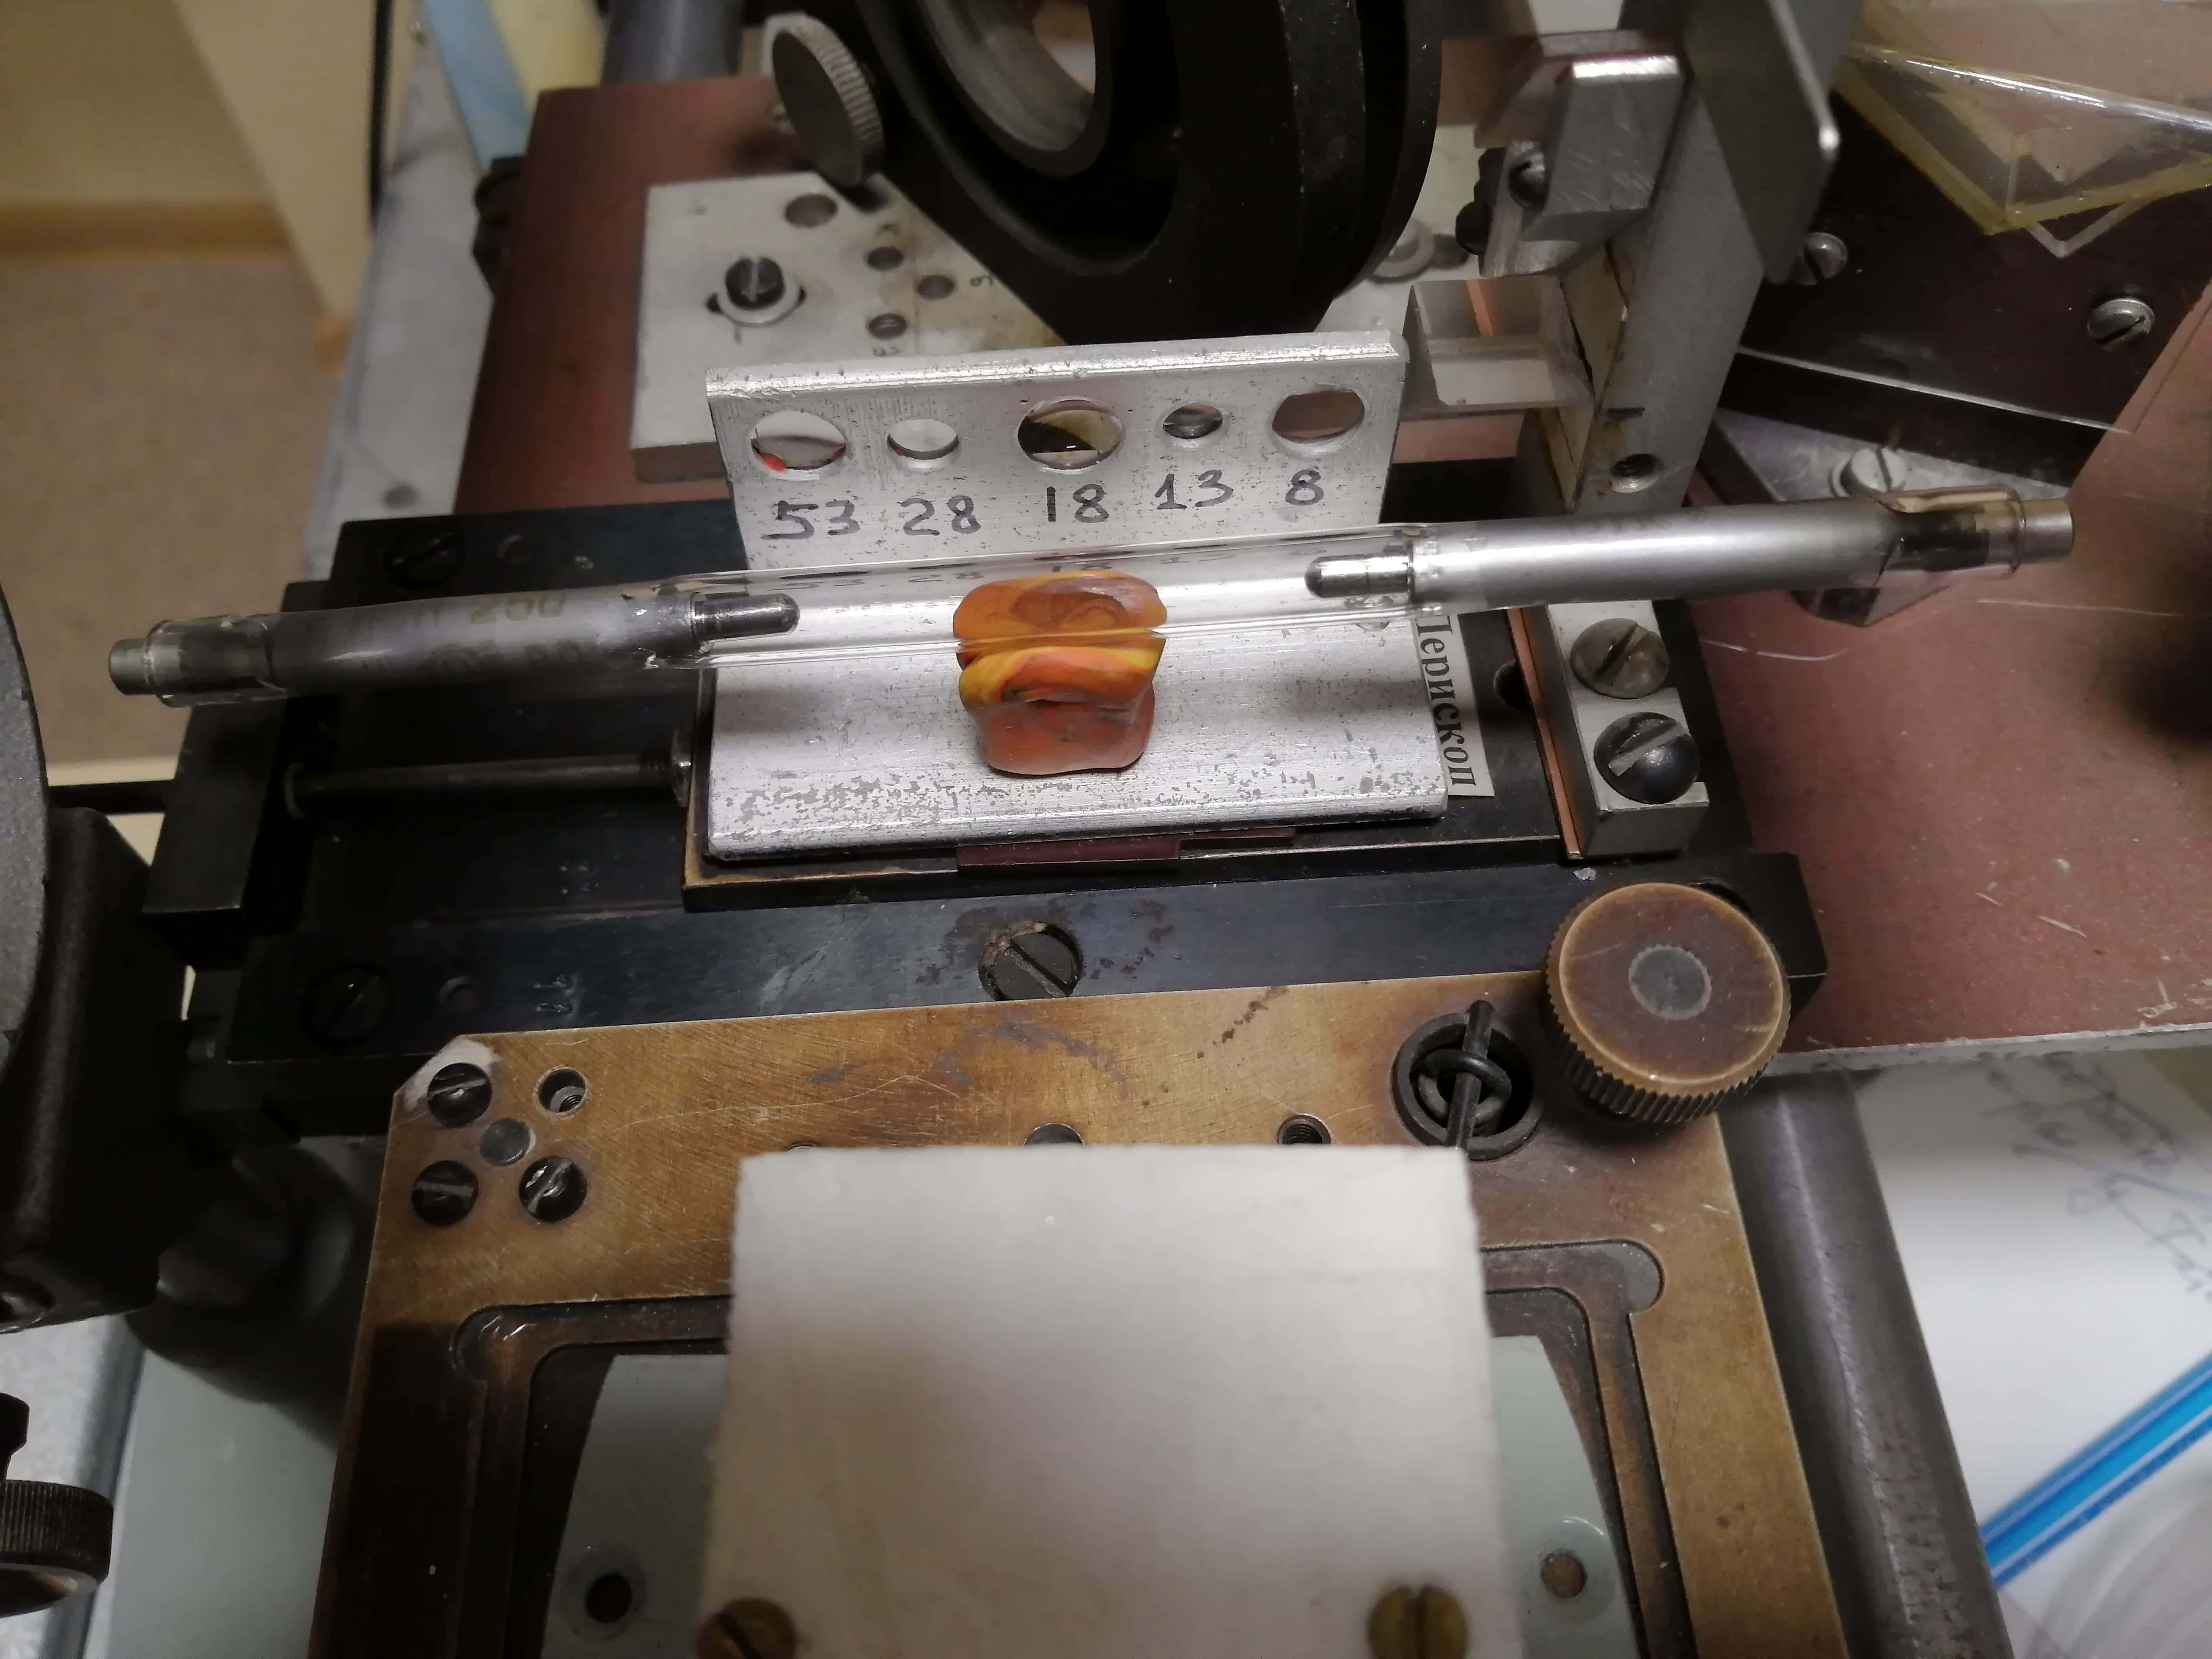
\includegraphics[width=\linewidth]{res/setup_lenses.png}
				\caption*{Площадка с набором линз для фокусировки пучка}
			\end{figure}
		\end{columns}
	\end{frame}	
	
	\begin{frame}
		\frametitle{Пробой воздуха}
		\begin{columns}
			\column{0.6\linewidth}
			\begin{figure}
				\centering
				\includegraphics[width=1\linewidth]{res/break_air_1mus_legend.png}
				\caption*{Интенсивность излучения от времени}
			\end{figure}	
			\column{0.4\linewidth}
			\begin{figure}
				\centering
				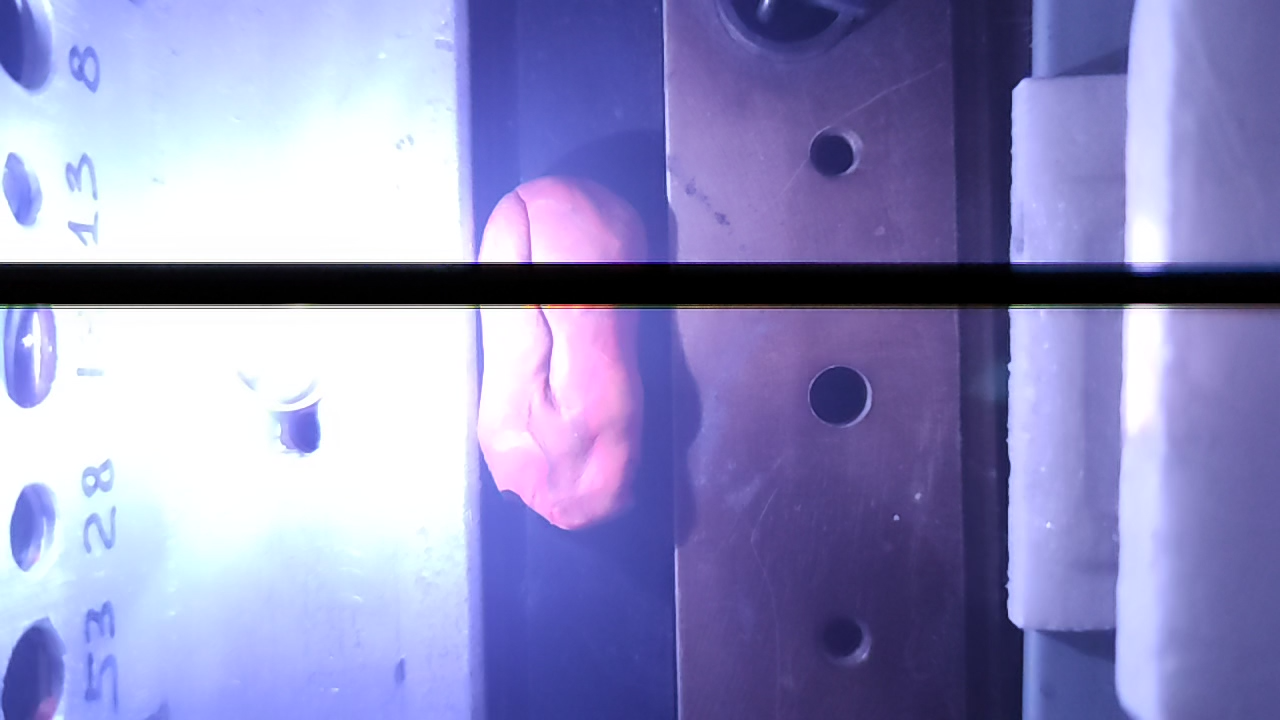
\includegraphics[width=\linewidth]{res/spark_air.png}
				\caption*{Фото пробоя}
			\end{figure}
		\end{columns}
	\end{frame}	
	
	\begin{frame}
		\frametitle{Спектр воздушного пробоя}
		\begin{figure}
			\centering
			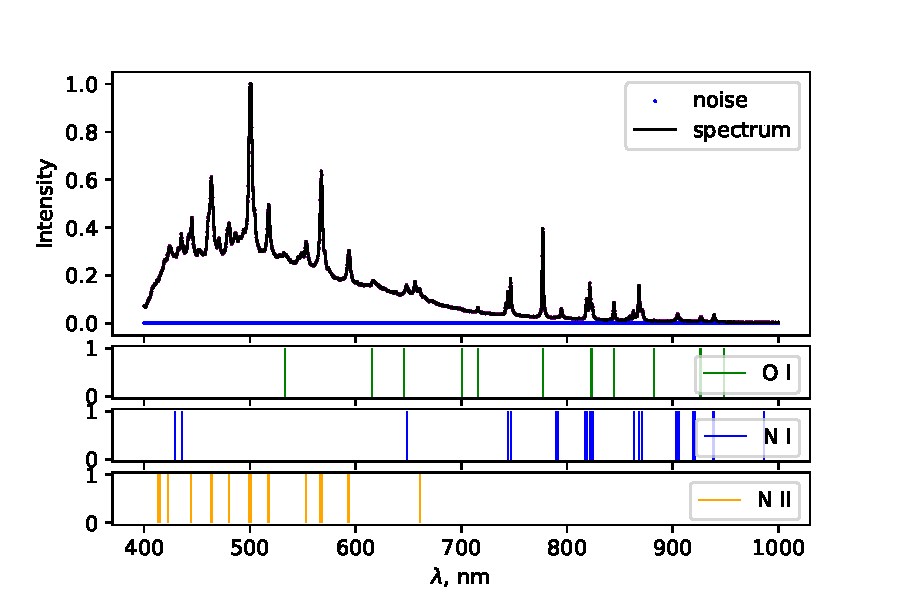
\includegraphics[width=\linewidth]{gen/air_lines.pdf}
			\caption*{Спектр пробоя в воздухе}
		\end{figure}
	\end{frame}

	\begin{frame}
		\frametitle{Пробой ксенона}
		\begin{columns}
			\column{0.6\linewidth}
			\begin{figure}
				\centering
				\includegraphics[width=1\linewidth]{res/break_spherical_1mus_legend.png}
				\caption*{Интенсивность излучения от времени}
			\end{figure}	
			\column{0.4\linewidth}
			\begin{figure}
				\centering
				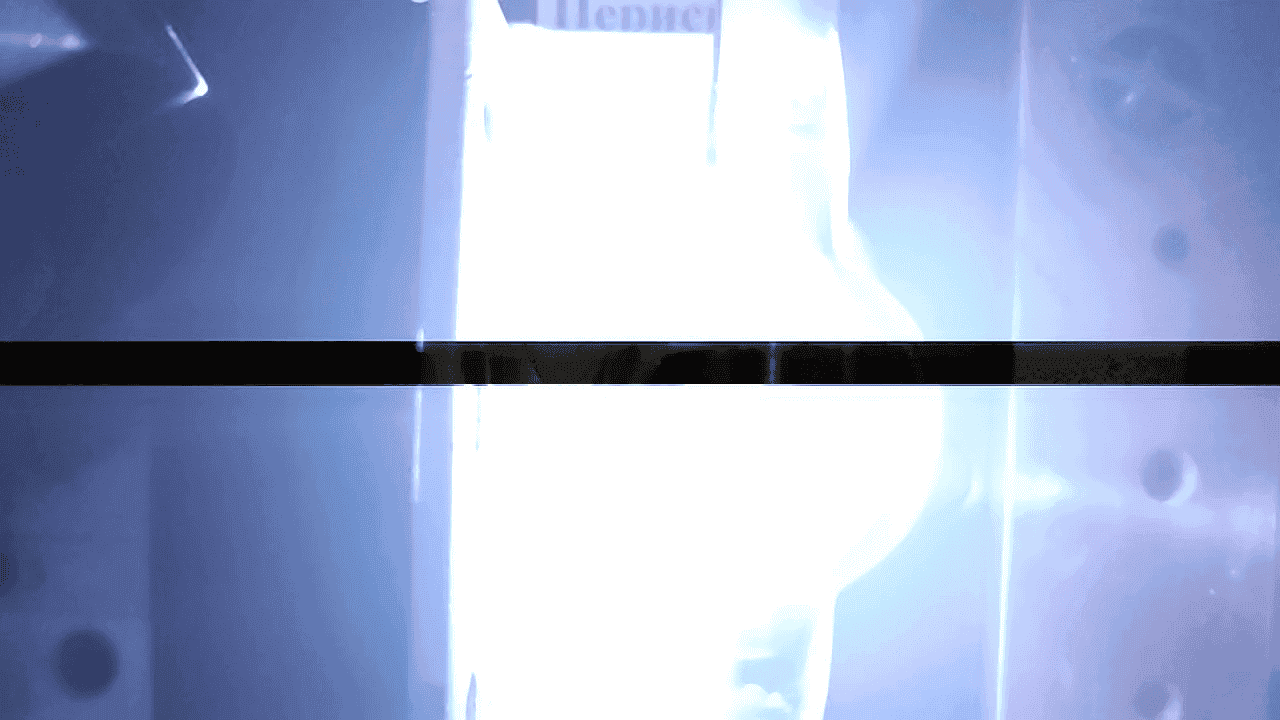
\includegraphics[width=\linewidth]{res/spark_spherical_xe.png}
				\caption*{Фото пробоя}
			\end{figure}
		\end{columns}
	\end{frame}	

	\begin{frame}
		\frametitle{Спектр пробоя ксенона}
		\begin{columns}
			\column{0.85\linewidth}
			\begin{figure}
				\centering
				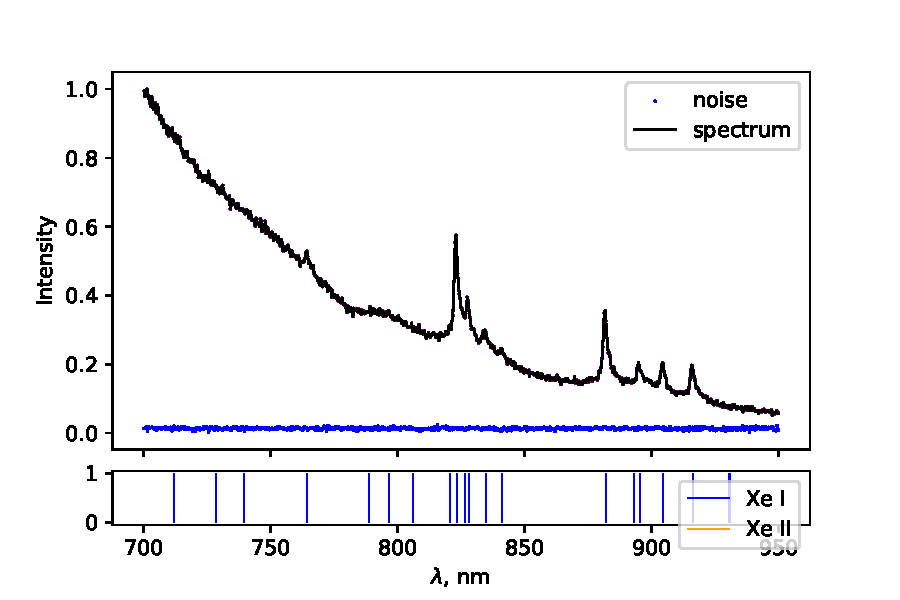
\includegraphics[width=1.1\linewidth]{gen/xe_lines_spherical.pdf}
				\caption*{Спектр пробоя ксенона}
			\end{figure}	
			\column{0.15\linewidth}
			\begin{figure}
				\centering
				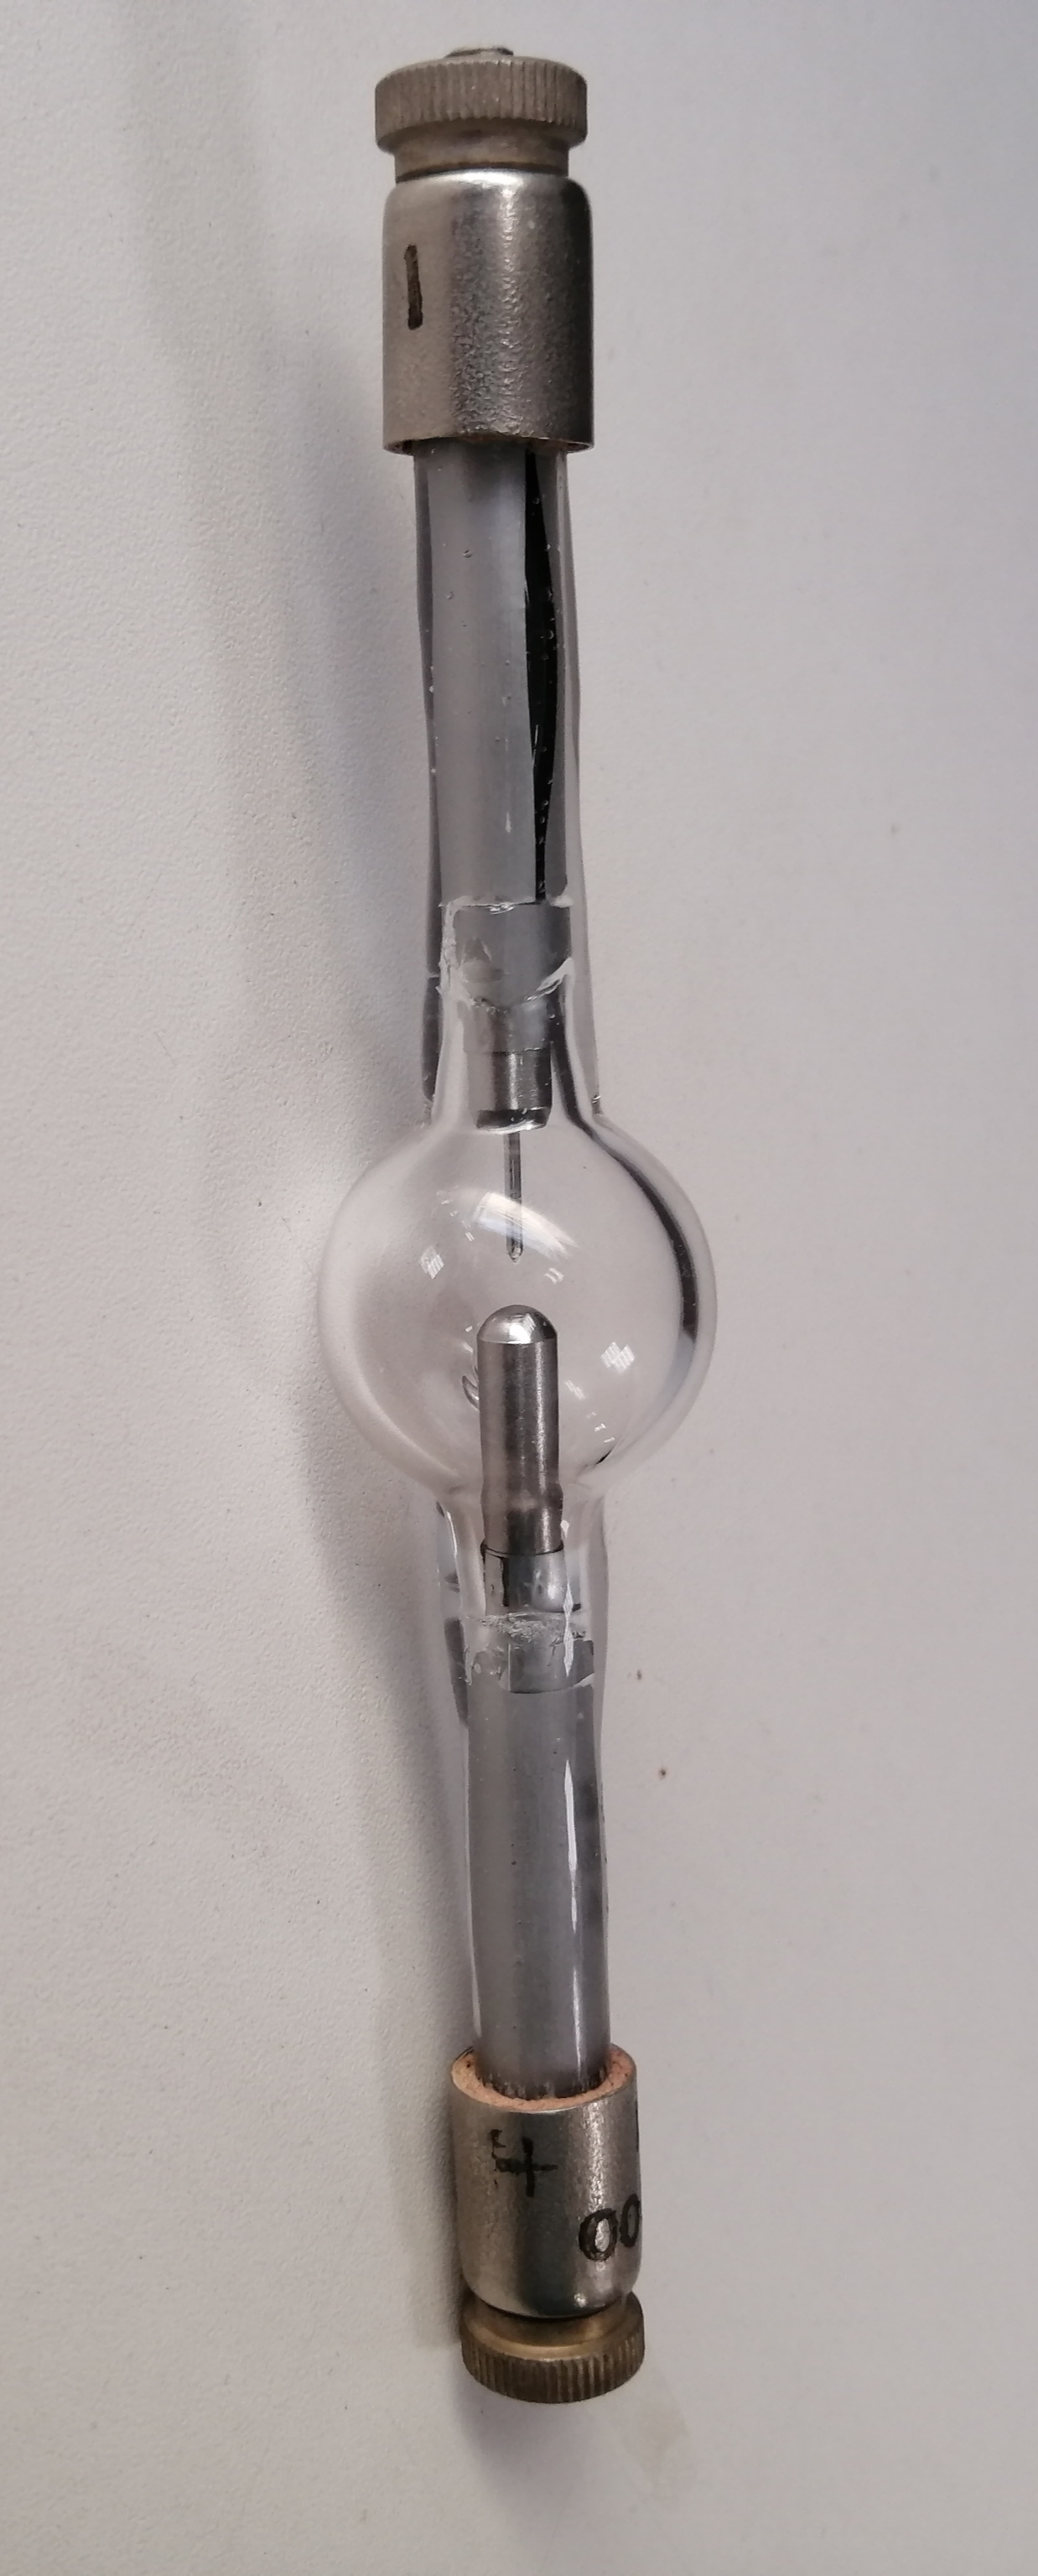
\includegraphics[width=\linewidth]{res/lamp_spherical_xe.png}
				\caption*{Шаровая лампа ДКСШ}
			\end{figure}
		\end{columns}
	\end{frame}	

		
	\begin{frame}
		\frametitle{Спектр пробоя ксенона}
		\begin{columns}
			\column{0.85\linewidth}
			\begin{figure}
				\centering
				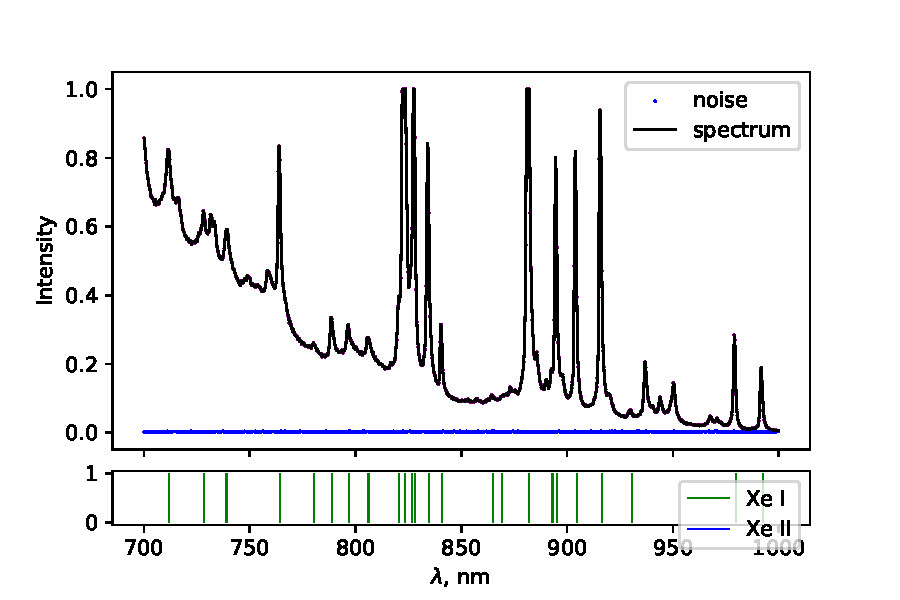
\includegraphics[width=1.1\linewidth]{gen/xe_lines.pdf}
				\caption*{Спектр пробоя ксенона}
			\end{figure}	
			\column{0.15\linewidth}
			\begin{figure}
				\centering
				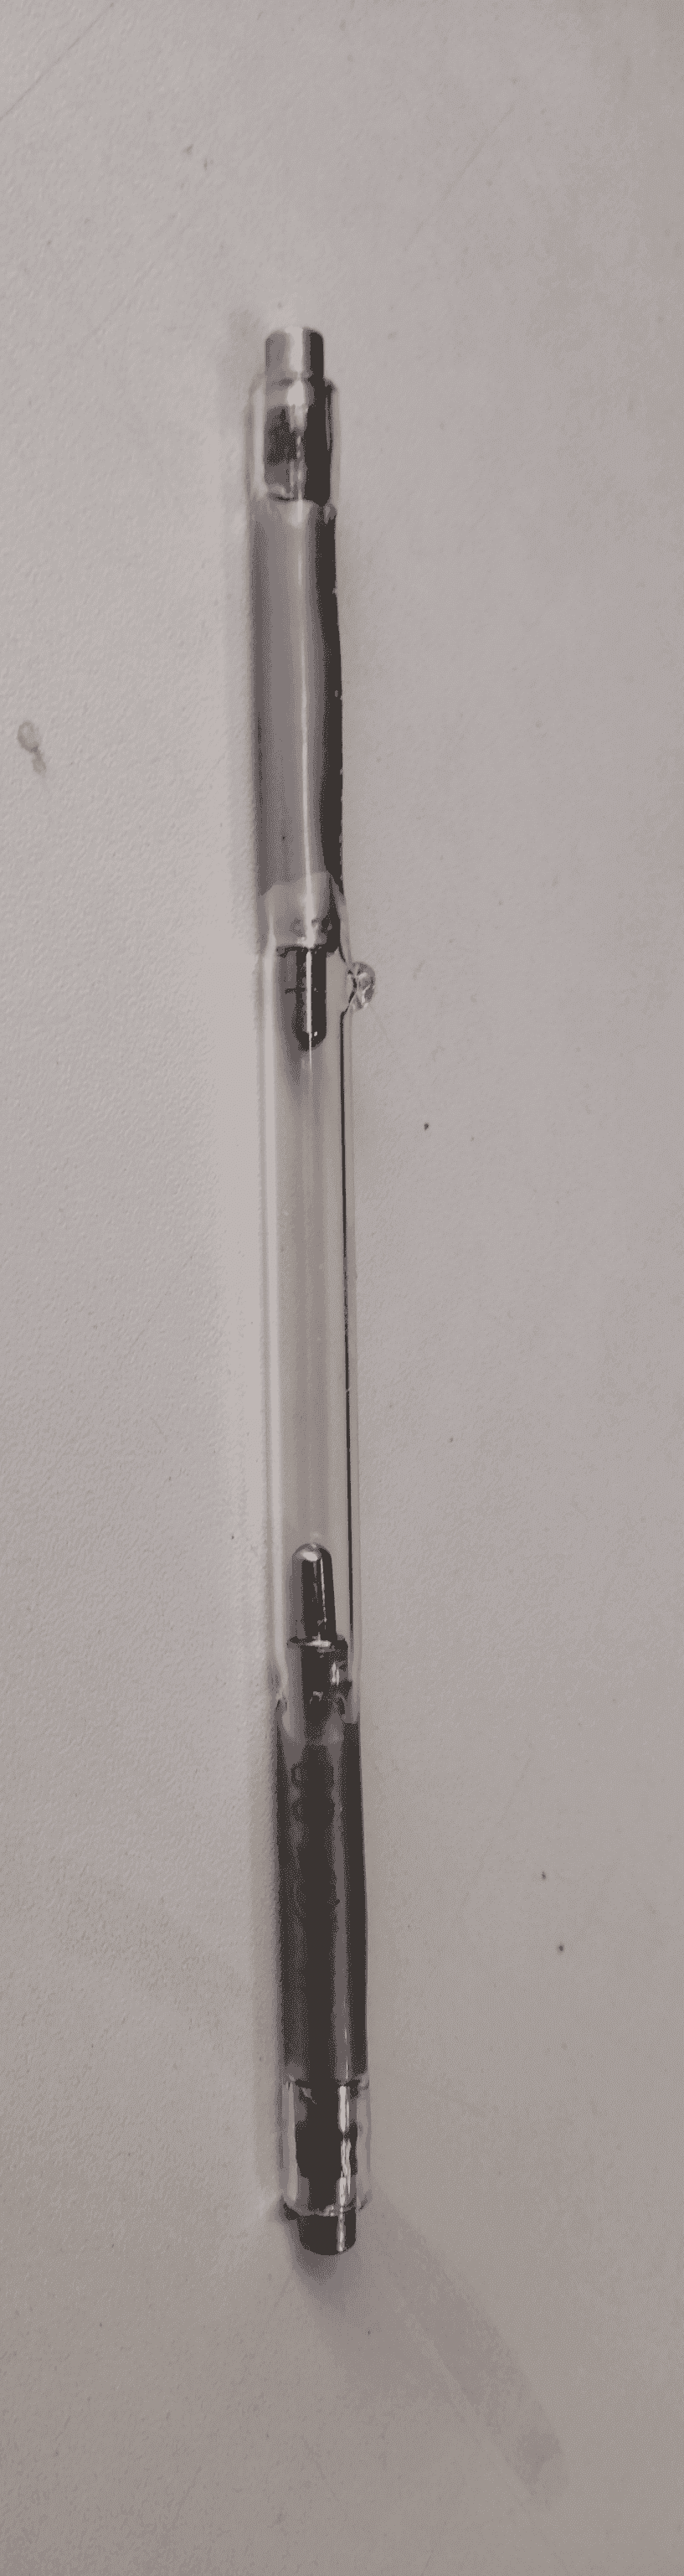
\includegraphics[width=\linewidth]{res/lamp_tube_xe.png}
				\caption*{Лампа ИФП-800}
			\end{figure}
		\end{columns}
	\end{frame}	

	\begin{frame}
		\frametitle{Спектр пробоя ксенона}
		\begin{columns}
			\column{0.85\linewidth}
			\begin{figure}
				\centering
				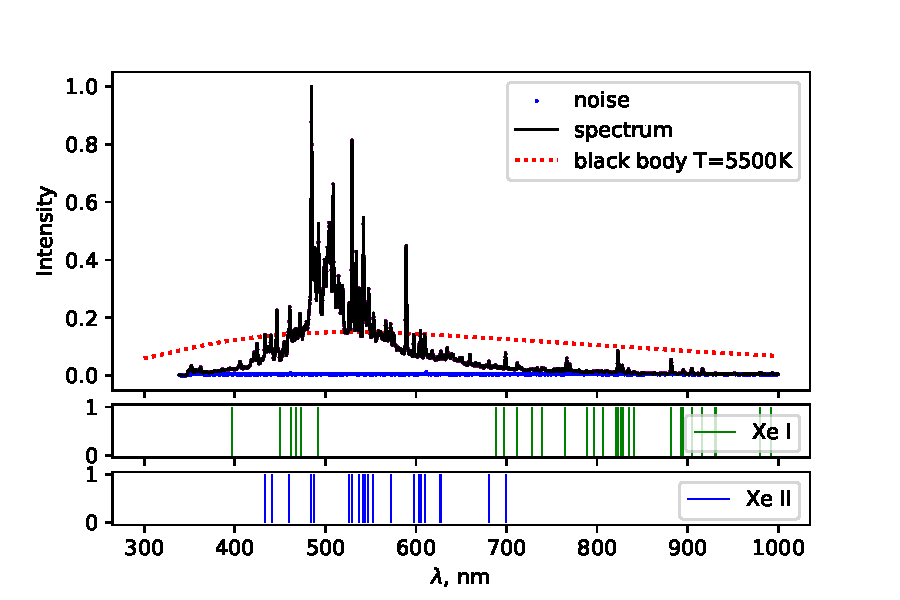
\includegraphics[width=1.1\linewidth]{gen/tirat_xe_lines.pdf}
				\caption*{Спектр пробоя ксенона}
			\end{figure}	
			\column{0.15\linewidth}
			\begin{figure}
				\centering
				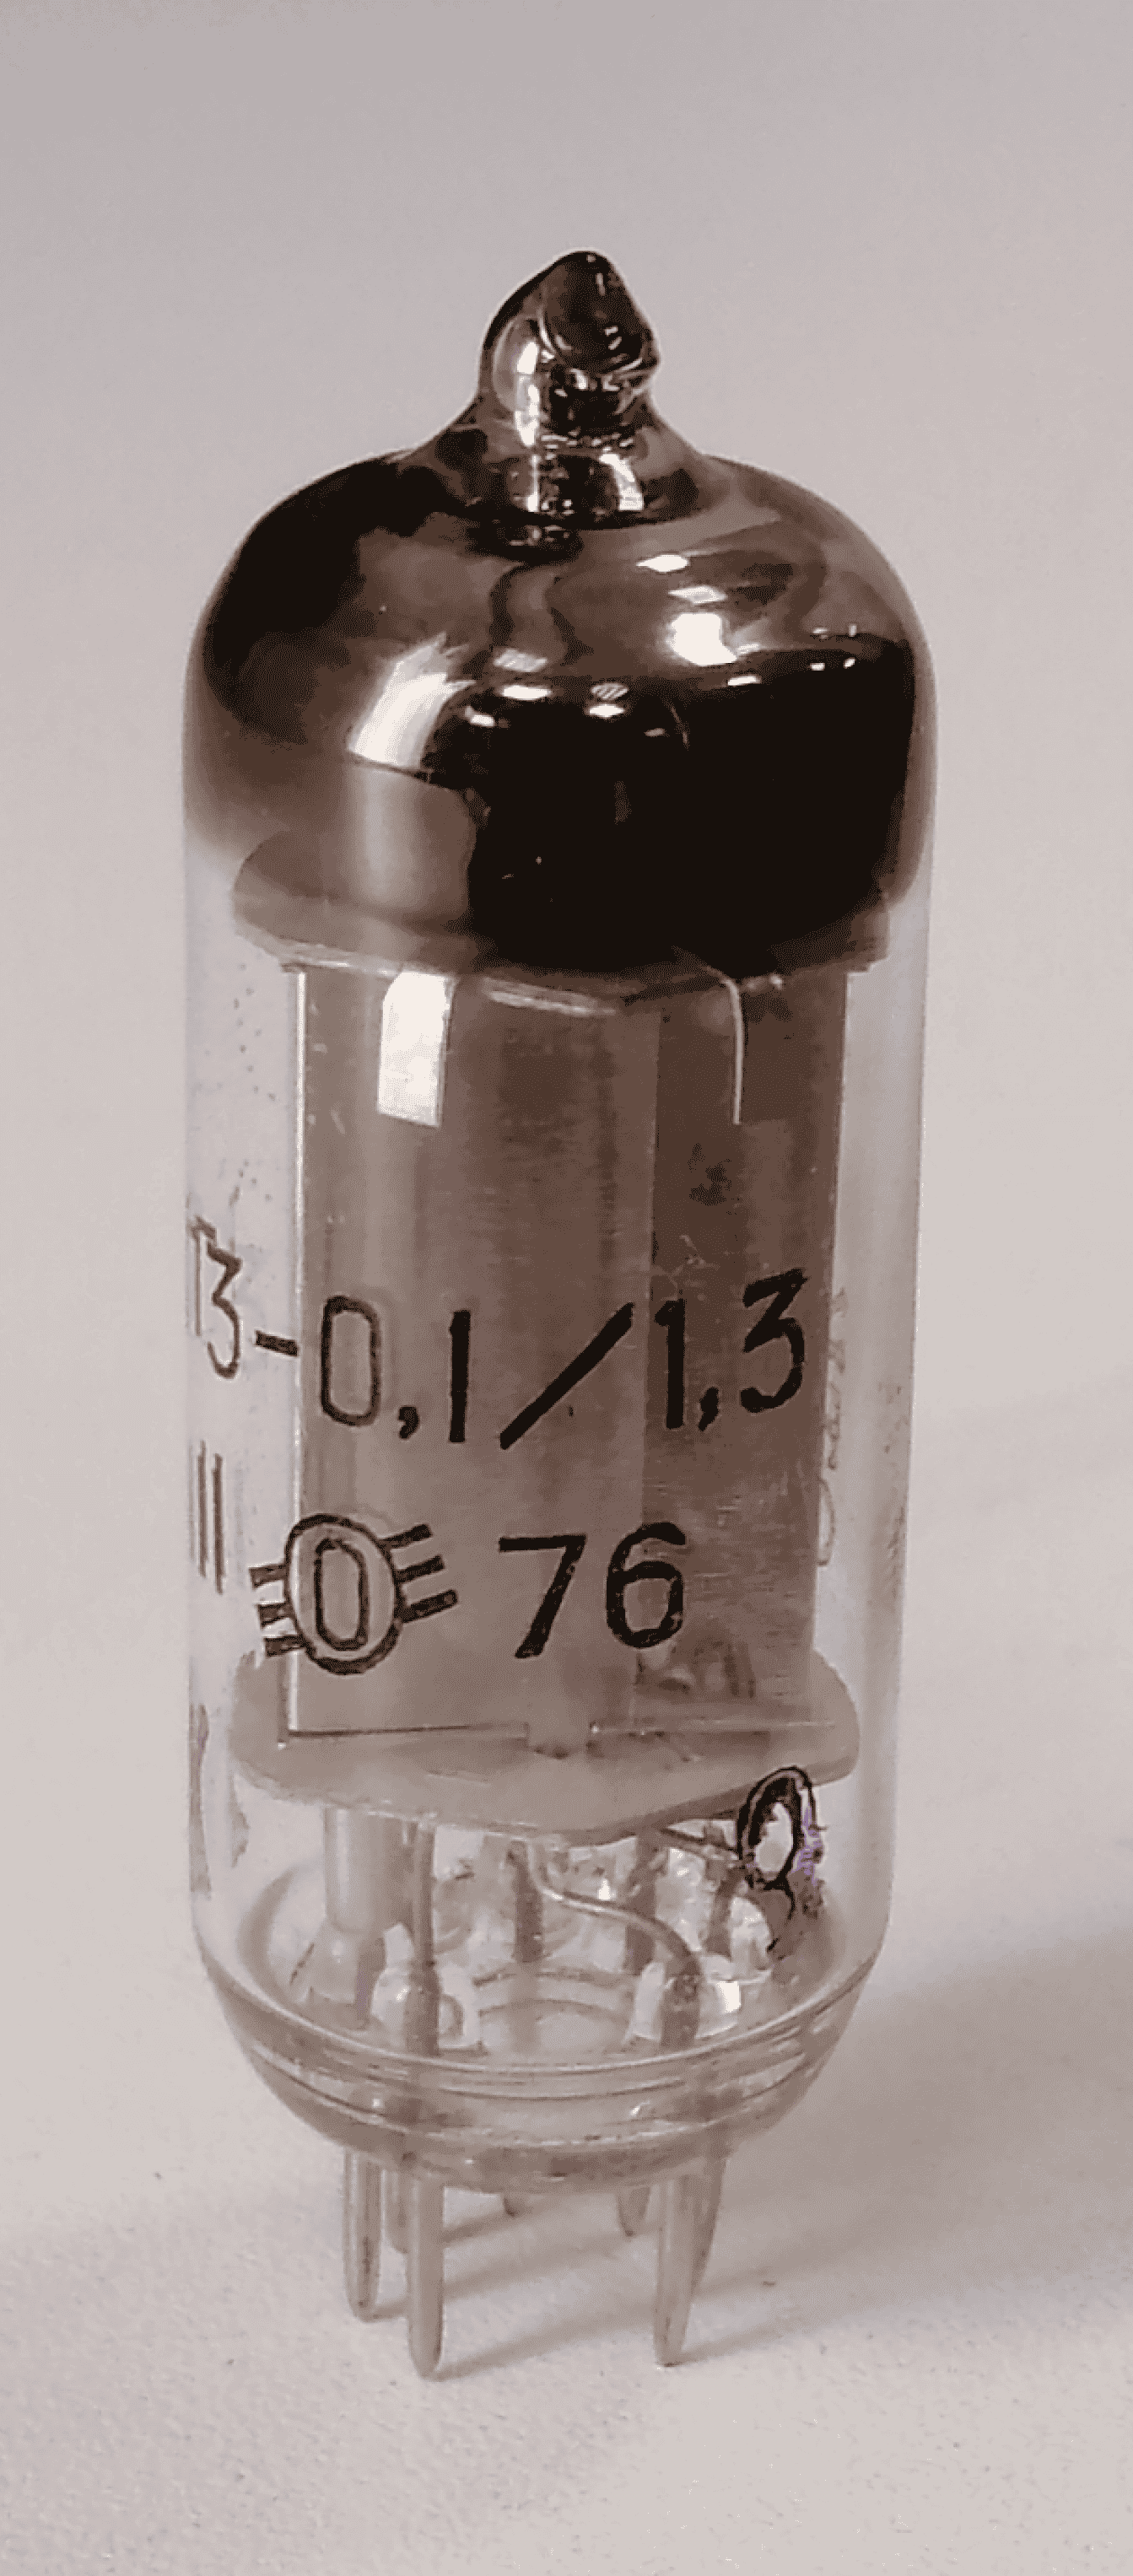
\includegraphics[width=\linewidth]{res/tirat_xe.png}
				\caption*{Тиратрон ТГ3-0.1/1.3}
			\end{figure}
		\end{columns}
	\end{frame}	

	\begin{frame}
		\frametitle{Спектр пробоя аргона}
		\begin{columns}
			\column{0.85\linewidth}
			\begin{figure}
				\centering
				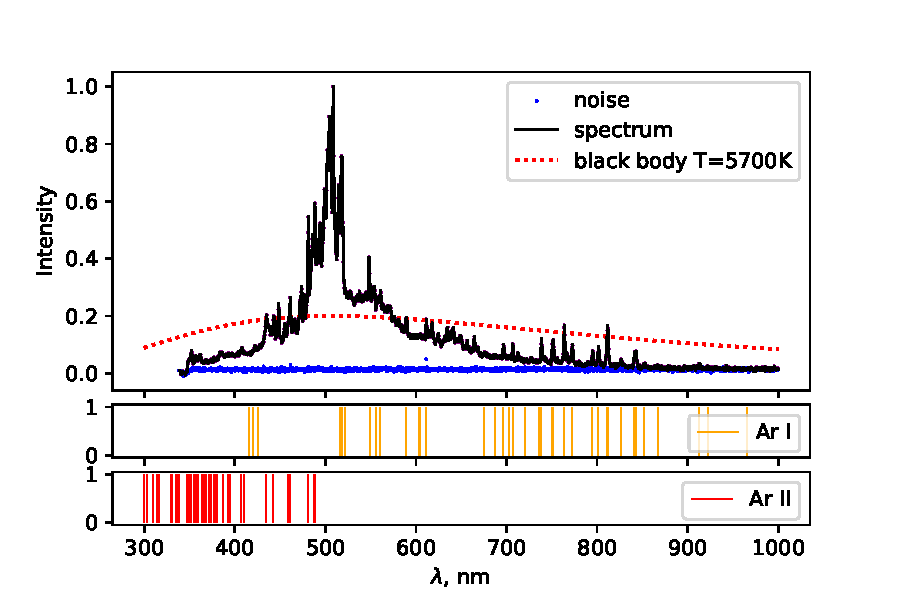
\includegraphics[width=1.1\linewidth]{gen/ar_lines.pdf}
				\caption*{Спектр пробоя аргона}
			\end{figure}	
			\column{0.15\linewidth}
			\begin{figure}
				\centering
				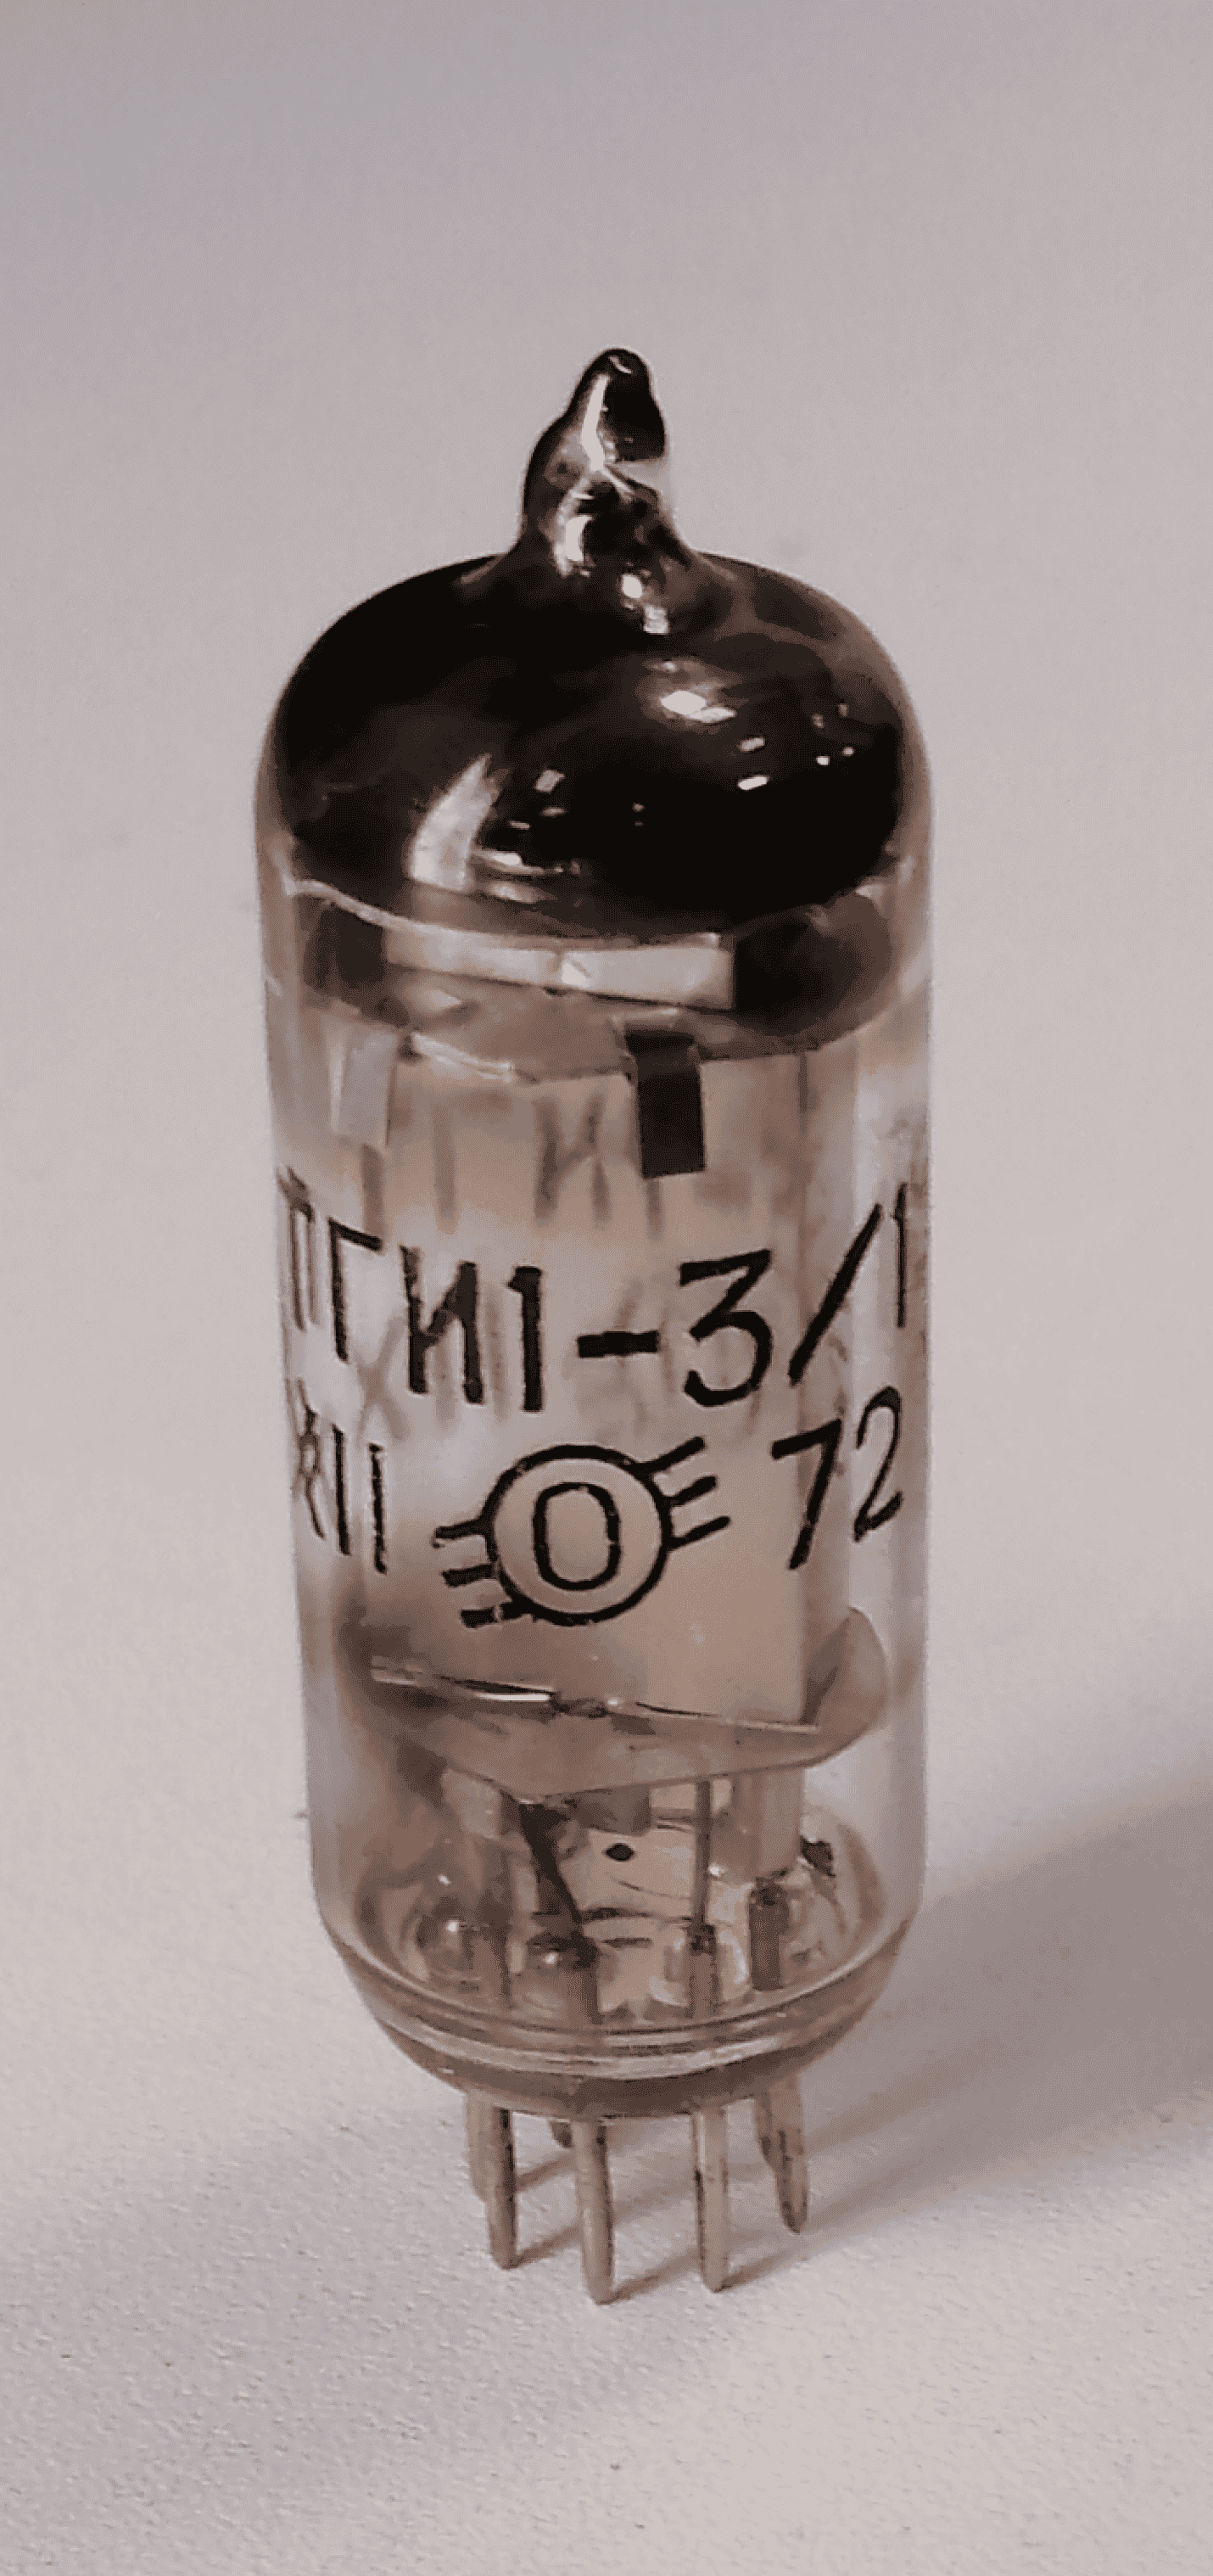
\includegraphics[width=\linewidth]{res/tirat_ar.png}
				\caption*{Тиратрон ТГИ1-3/1}
			\end{figure}
		\end{columns}
	\end{frame}	

	\begin{frame}
		\frametitle{Пробой воды}
		\begin{columns}
			\column{0.6\linewidth}
			\begin{figure}
				\centering
				\includegraphics[width=1\linewidth]{res/break_water_500ns_legend.png}
				\caption*{Интенсивность излучения от времени}
			\end{figure}	
			\column{0.4\linewidth}
			\begin{figure}
				\centering
				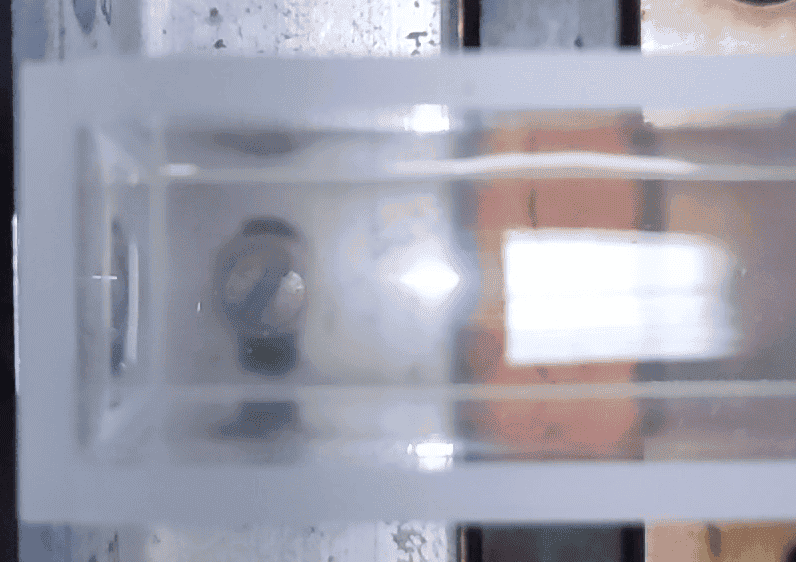
\includegraphics[width=\linewidth]{res/water_spark.png}
				\caption*{Фото пробоя}
			\end{figure}
		\end{columns}
	\end{frame}	

	\begin{frame}
		\frametitle{Спектр пробоя воды}
		\begin{columns}
			\column{0.85\linewidth}
			\begin{figure}
				\centering
				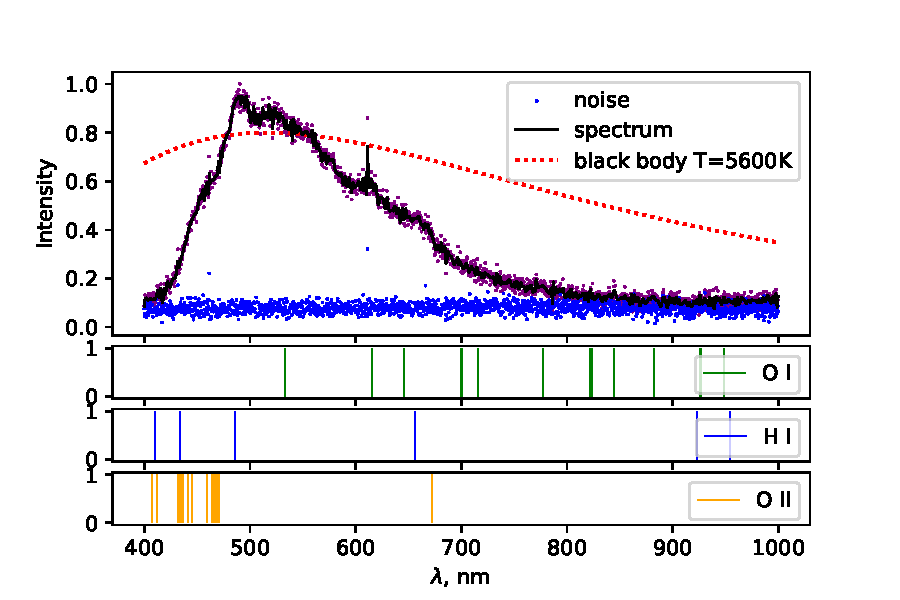
\includegraphics[width=1.1\linewidth]{gen/water_lines.pdf}
				\caption*{Спектр пробоя воды}
			\end{figure}	
			\column{0.15\linewidth}
			\begin{figure}
				\centering
				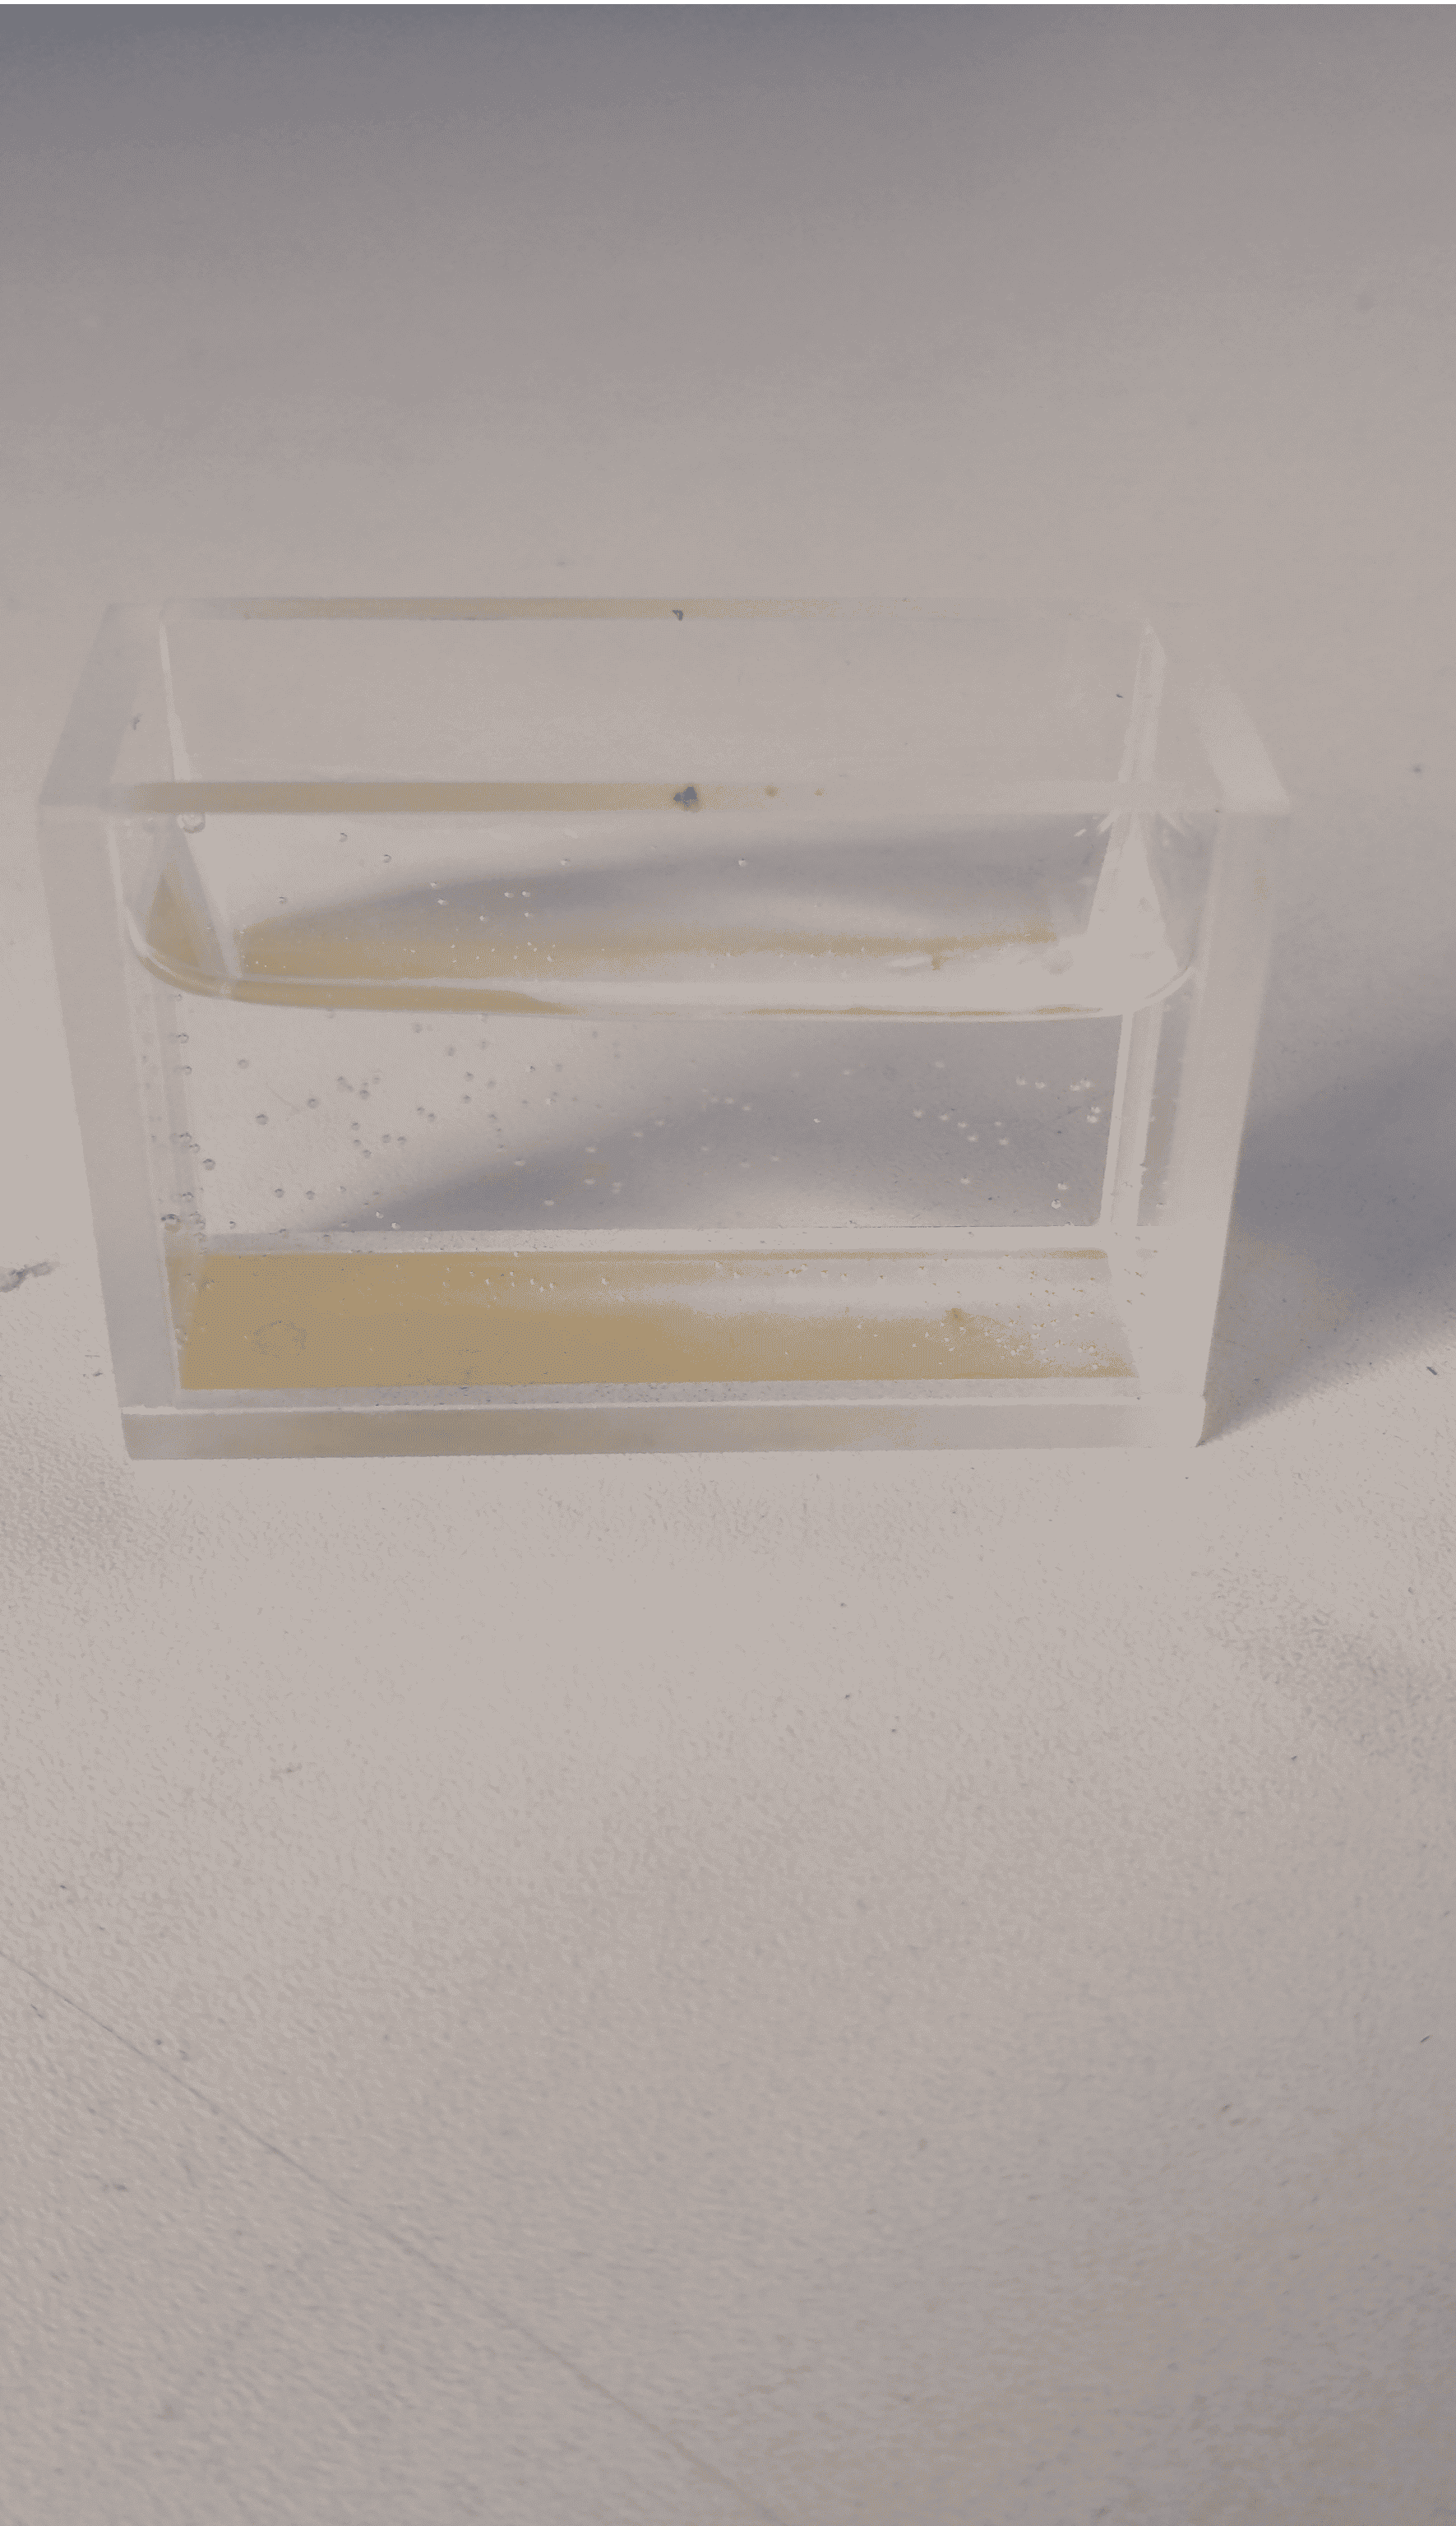
\includegraphics[width=\linewidth]{res/water_cuvette.png}
				\caption*{Кювета с водой}
			\end{figure}
		\end{columns}
	\end{frame}	

	\begin{frame}
		\frametitle{Оценка пороговой интенсивности}
		\begin{columns}
			\column{0.3\linewidth}
			\begin{figure}
				\centering
				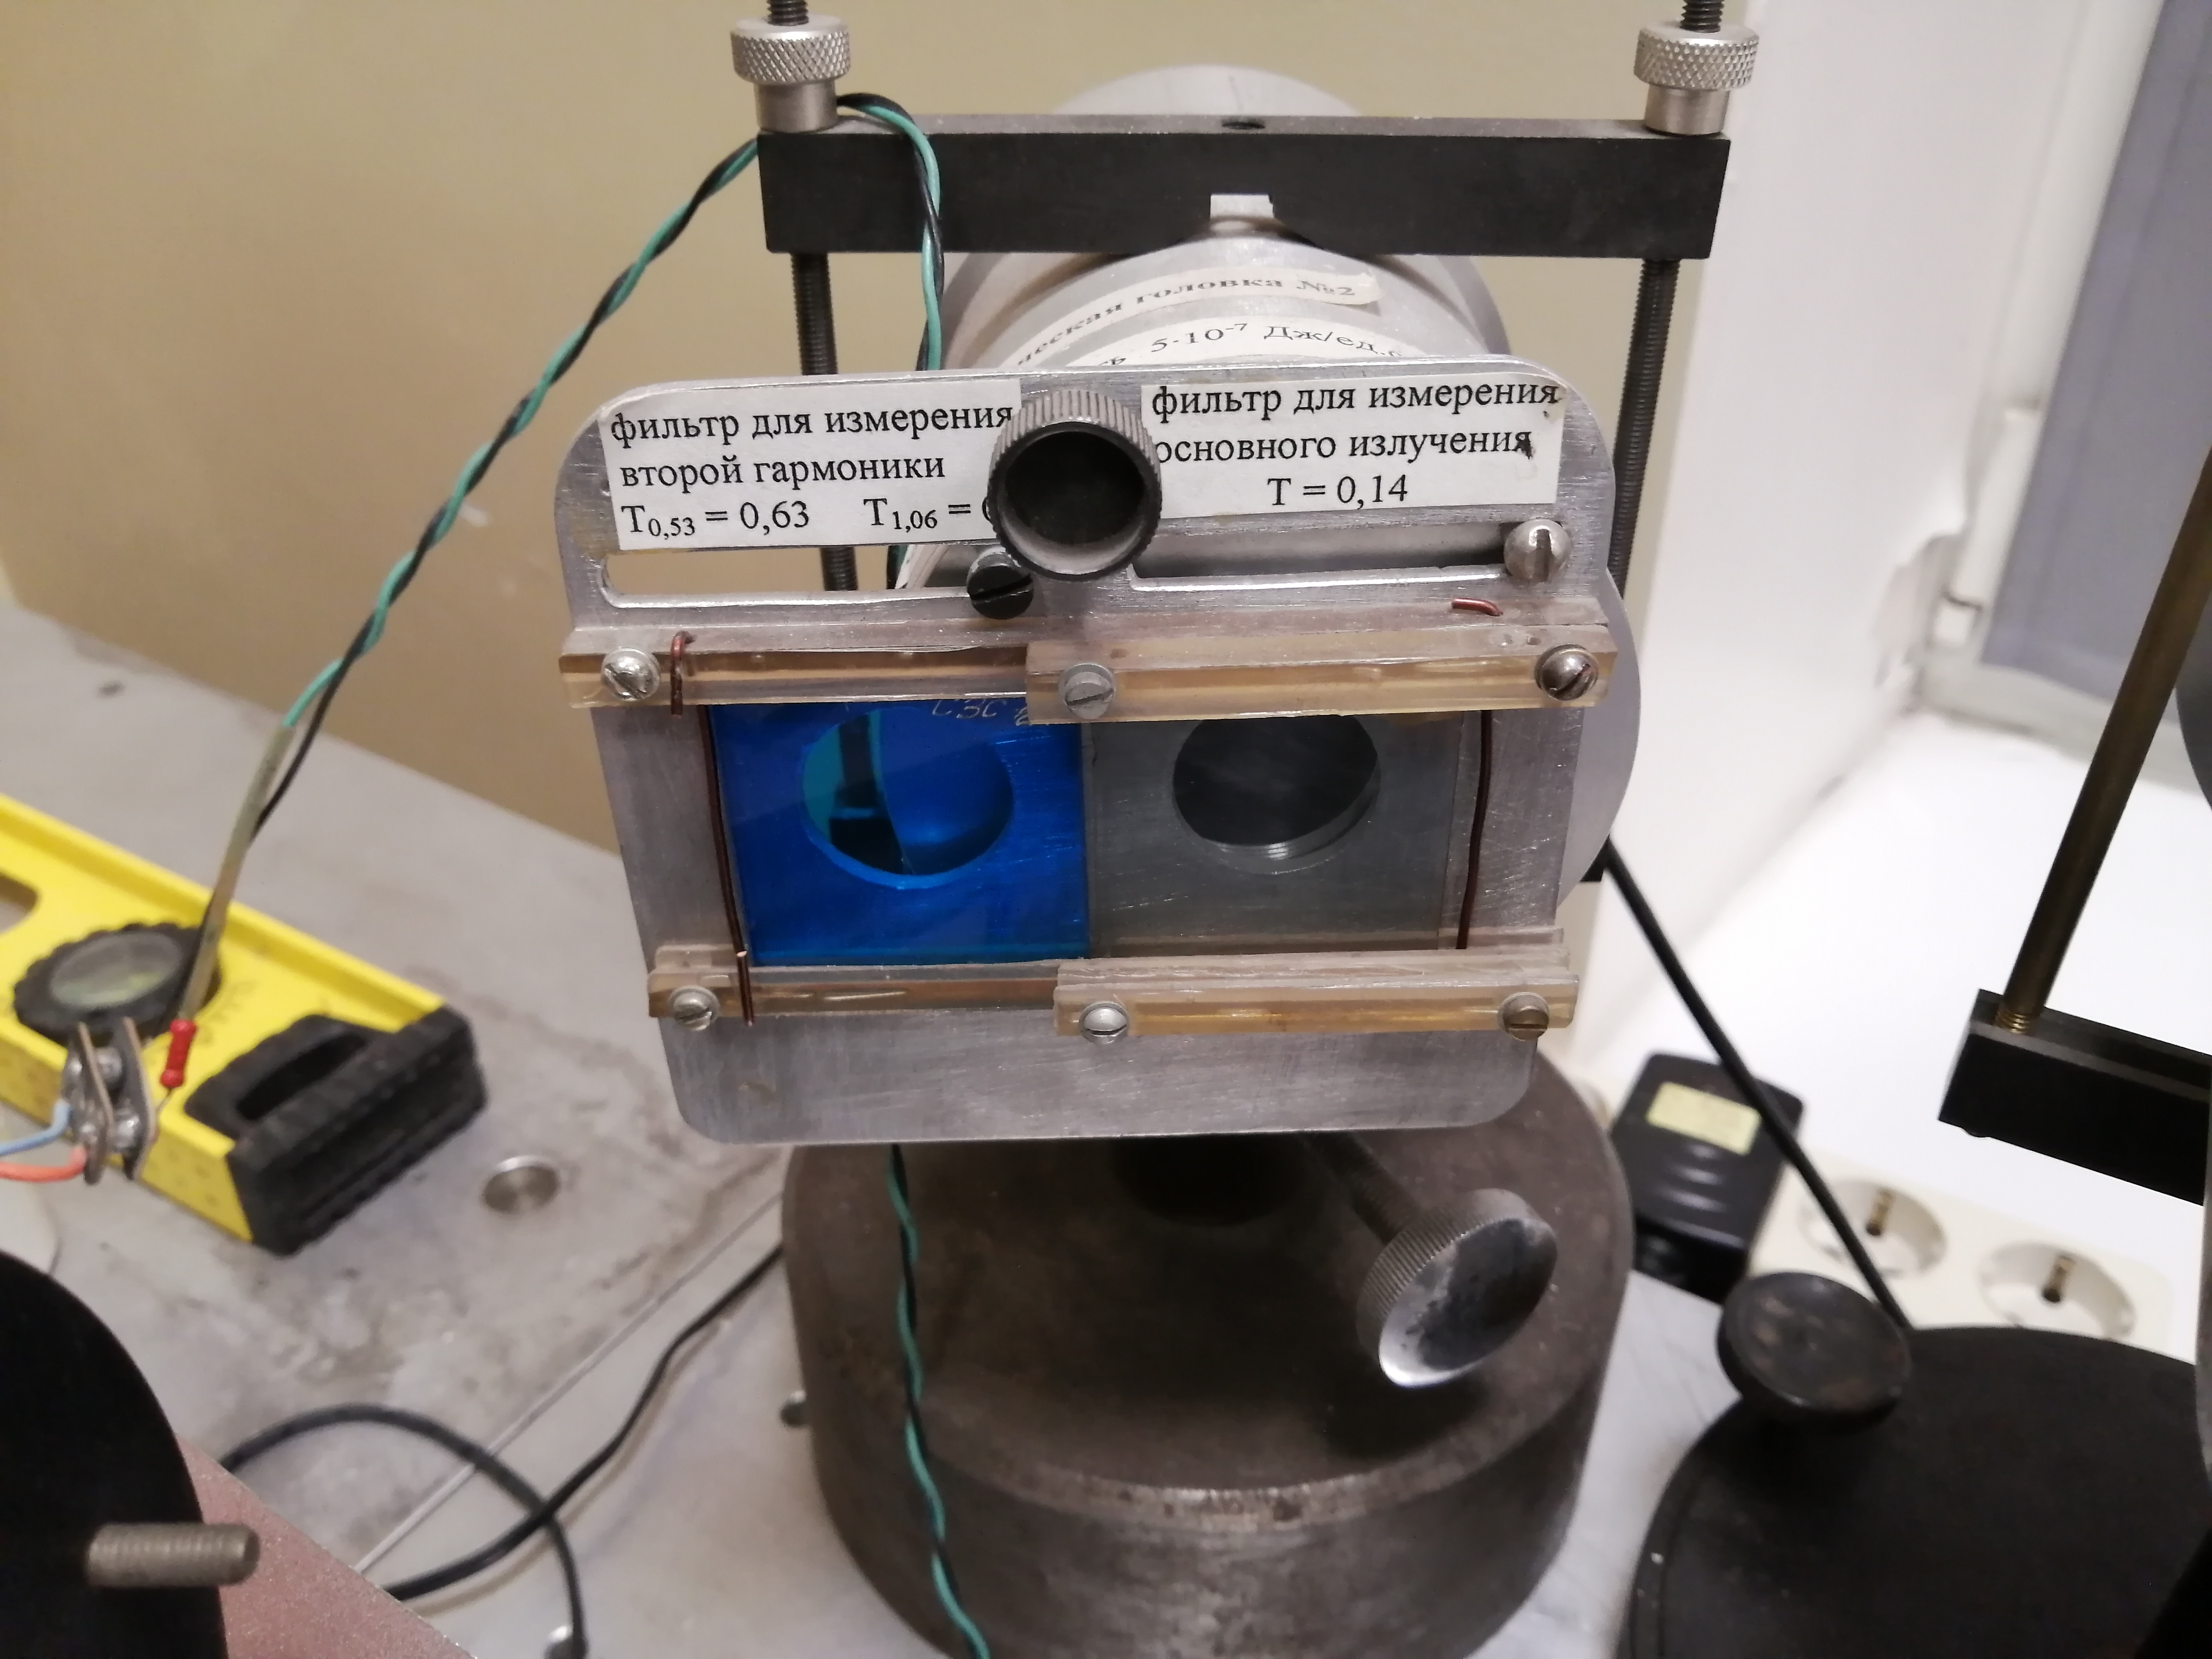
\includegraphics[width=1\linewidth]{res/calorimeter.png}
				\caption*{Фото калориметра}
			\end{figure}	
			\column{0.7\linewidth}
			\vspace{5pt}
			Пороговое значение энергии лазера, измеренное калориметром: 
			$$W = (0.08 \pm 0.01) \text{ Дж}.$$
			
			Диаметр пятна в фокусе линзы: 
			$$d = \theta f = (54 \pm 16) \text{ мкм},$$
			$\theta \approx 3.0 \cdot 10^{-3} \text{ рад.}$ -- угловая расходимость лазерного пучка, \\
			$f = 18 \text{ мм}$ -- фокусное расстояние линзы. \\
		\end{columns}
	\end{frame}	

	\begin{frame}
		\frametitle{Оценка пороговой интенсивности}
		\vspace{5pt}
		Оценка пороговой интенсивности: 
		$$S_{\text{min}} = \Theta \cdot \frac{W}{ \tau \left(\frac{\pi d^2}{4}\right)} = (1.8 \pm 0.6)\cdot10^{11} \frac{\text{Вт}}{\text{см}^2},$$
		$\tau = 40 \text{ нс}$ -- время импульса, \\
		$\Theta \sim 2$ -- коэффициент формы импульса.
		
		\begin{figure}
			\centering
			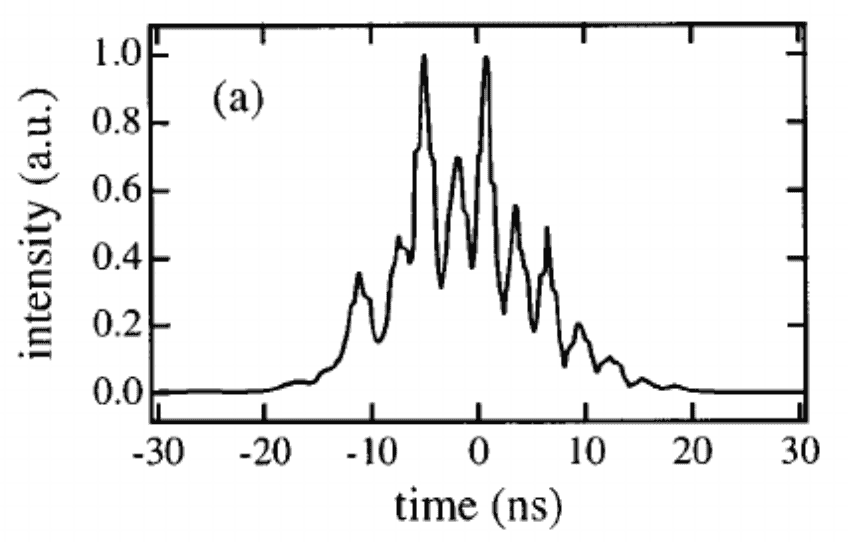
\includegraphics[width=0.5\linewidth]{res/qswitched_pulse_form.png}
			\caption*{Временная форма импульса неодимового лазера с Q-модуляцией}
		\end{figure}	
		
	\end{frame}	

	\begin{frame}[plain,c]
		
		\begin{center}
			\huge \usebeamercolor[fg]{frametitle} Выводы и Заключение
		\end{center}
		
	\end{frame}

	\begin{frame}
		\frametitle{Выводы}
		\begin{itemize}
			\item Был изучен лазерный пробой. Пороговые значения поля были измерены:
			$$ E_{air} = 8.2 \cdot 10^6 \text{ V/cm}$$
			\item Теоретические оценки согласуются с экспериментальными данными.
			\footnotesize
			\begin{table}[]
				\begin{tabular}{llll}
					\hline
					& Ксенон            & Аргон            & Воздух              \\ \hline
					Эксперимент\footnote{According to: \cite{raizer}, \cite{argon_threshold}, \cite{xenon_threshold}, \cite{air_breakdown}, \cite{air_threshold}}, V/cm & $(1.5 \div 2.3) \cdot 10^6$ & $(2.7 \div 3.1) \cdot 10^6$ & $(5 \div 13) \cdot 10^6$ \\
					Оценка, V/cm & $1.5 \cdot 10^6$ & $2.7 \cdot 10^6$ & $2.4 \cdot 10^6$ \\ \hline
				\end{tabular}
			\end{table}
			
			\item 
			\normalsize Были собраны спектры и временные характеристики пробоя.
			\begin{columns}
				\column{0.33\linewidth}
				\begin{figure}
					\centering
					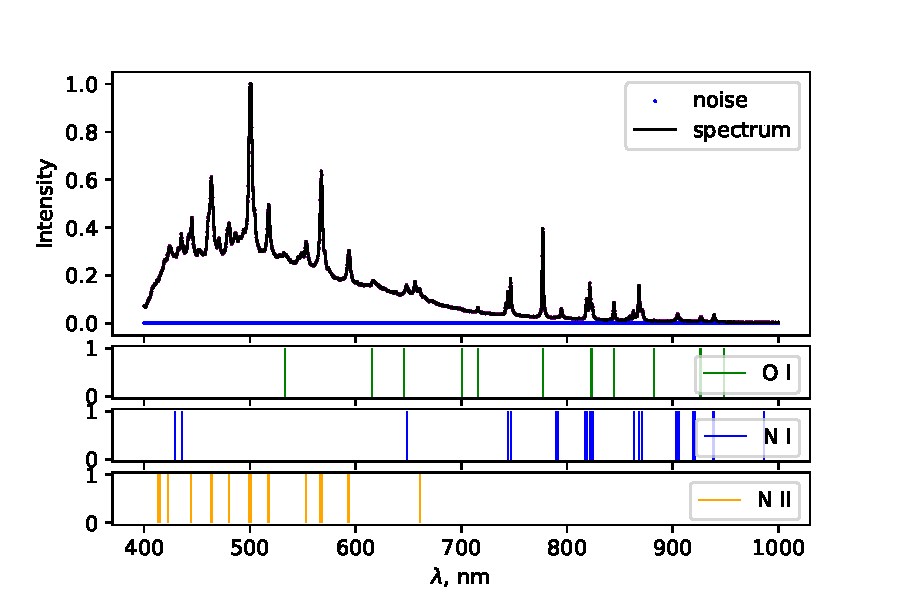
\includegraphics[width=\linewidth]{gen/air_lines.pdf}
					\caption*{Спектр воздуха}
				\end{figure}
				
				\column{0.33\linewidth}
				\begin{figure}
					\centering
					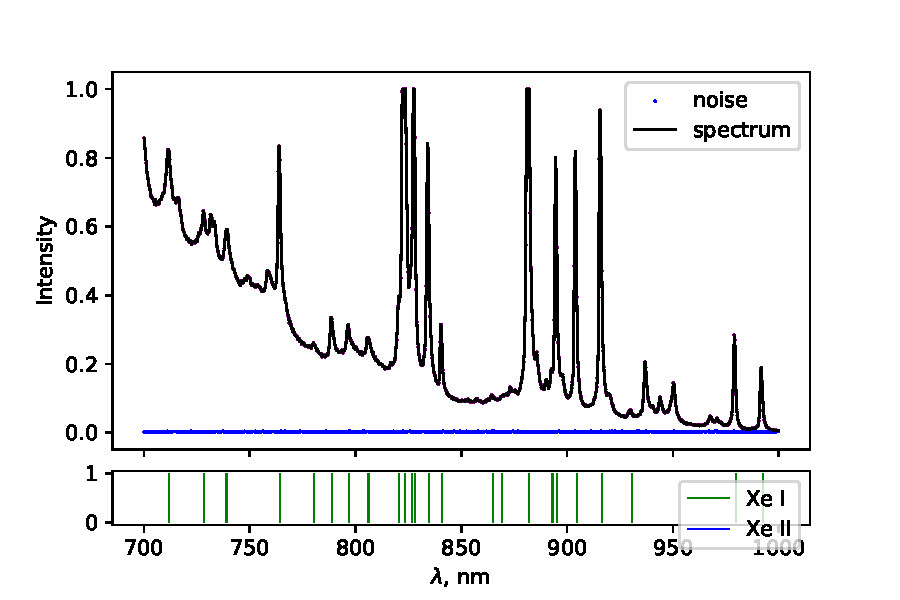
\includegraphics[width=\linewidth]{gen/xe_lines.pdf}
					\caption*{Спектр ксенона}
				\end{figure}
				
				\column{0.33\linewidth}
				\begin{figure}
					\centering
					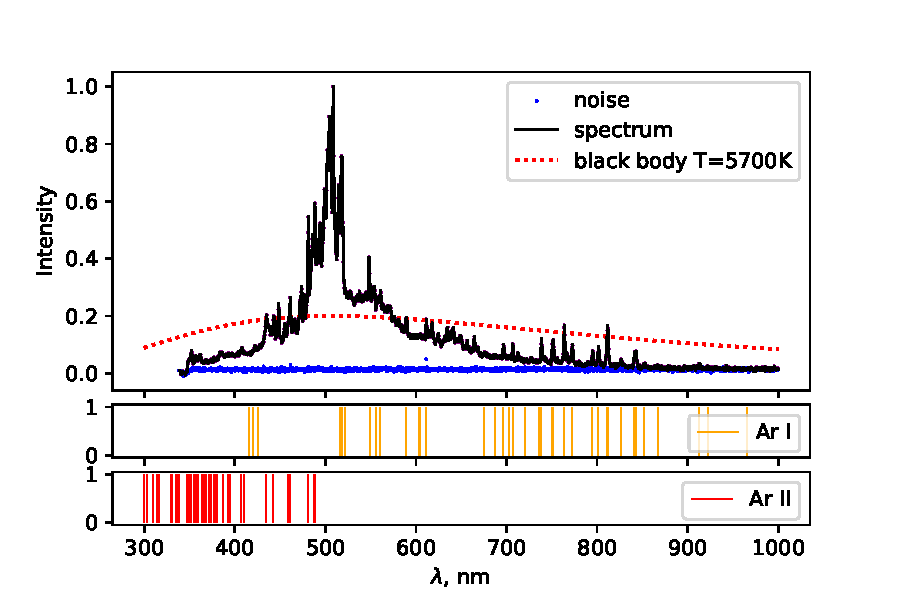
\includegraphics[width=\linewidth]{gen/ar_lines.pdf}
					\caption*{Спектр аргона}
				\end{figure}
				
			\end{columns}
			
		\end{itemize}
		
	\end{frame}
	
	\begin{frame}
		\frametitle{Улучшения}
		В дальнейшем можно:
		\begin{itemize}
			\item Использовать фотодиод с более высоким временным разрешением.
			\item Фотографировать пробой на CCD/ICCD камеру.
			\item Проводить измерения в оптической кювете.
			\item Применить более точную теорию для оценок.
		\end{itemize}
		
		\begin{columns}
			\column{0.5\linewidth}
			\begin{figure}
				\centering
				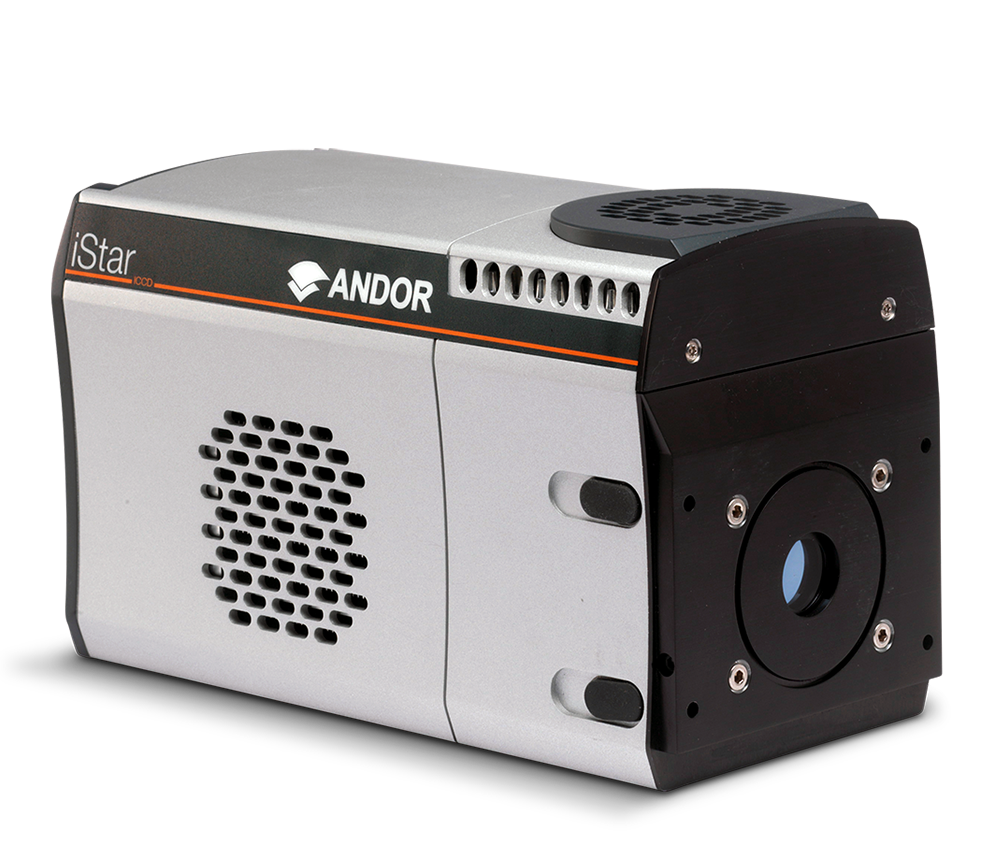
\includegraphics[width=0.9\linewidth]{res/iccd_camera.png}
				\caption*{ICCD camera}
			\end{figure}
			\column{0.5\linewidth}
			\begin{figure}
				\centering
				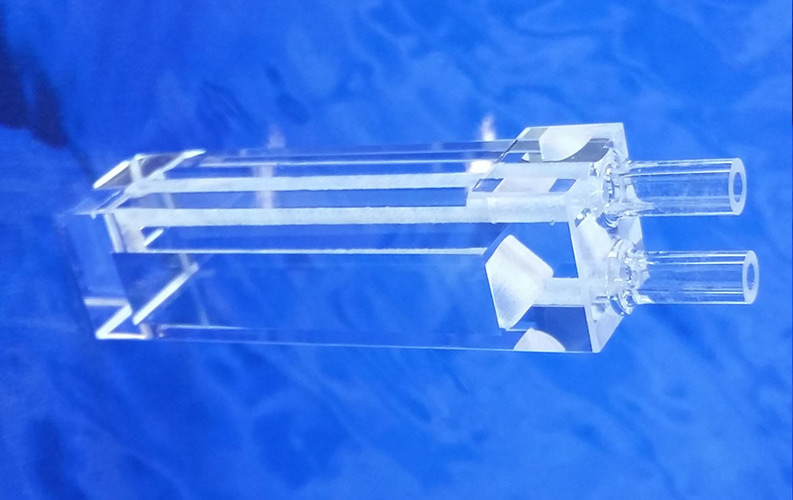
\includegraphics[width=0.9\linewidth]{res/gas_cuvette.jpeg}
				\caption*{Optical gas cuvette}
			\end{figure}
		\end{columns}
		
		
	\end{frame}
	
	\begin{frame}[plain,c]
		
		\begin{center}
			\huge \usebeamercolor[fg]{frametitle} Спасибо за внимание!
		\end{center}
		
	\end{frame}
	
	\begin{frame}
		\frametitle{Приложение: Пороговые значения пробоя в воздухе.}
		
		\begin{figure}
			\centering
			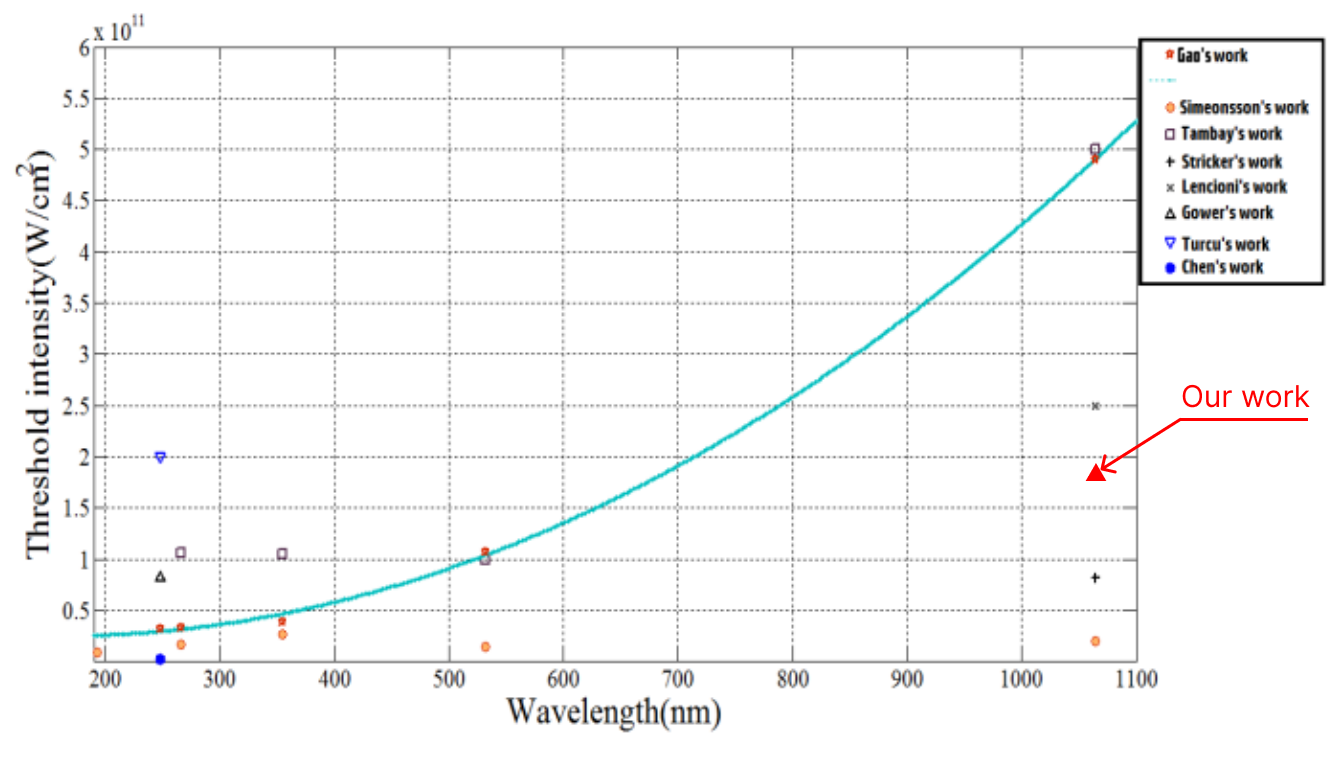
\includegraphics[width=\linewidth]{res/air_threshold_variety.png}
			\caption*{Variety of threshold fields}
		\end{figure}
	\end{frame}
	
	\begin{frame}
		\begin{thebibliography}{99} % Bibliography - this is intentionally simple in this template
			\footnotesize
			\bibitem{raizer}
			Y. P. Raizer, 'Laser Spark and Propagation of Discharges'.
			
			\bibitem{spark_evolution}
			S. S. Harilal, B. E. Brumfield, M. C. Phillips, 'Lifecycle of laser-produced air sparks'.
			
			\bibitem{air_breakdown}
			Kai-Ting Yen, Chih-Hung Wu, Pin-Hsun Wang, Pi-Hui Tuan, Kuan-Wei Su, 'Investigating the Threshold Conditions of Air Breakdown
			with Mode-Locked Q-Switched Laser Pulses, and the Temporal
			Dynamics of Induced Plasma with Self-Scattering Phenomenon'
			
			\bibitem{argon_threshold}
			F. Morgan, 'Laser beam induced breakdown in helium and
			argon'.
			
			\bibitem{xenon_threshold}
			Yosr E. E-D. Gamal, M. A. Mahmoud, Nagia Dawood, 'Numerical investigation of the threshold intensity dependence on gas pressure in the breakdown of xenon by different laser wavelengths'.
			
			\bibitem{air_threshold}
			Zhixing Gao, Lixuan Hana, Jing Lia, 'Investigation of laser induced air breakdown thresholds at 1064, 532, 355, 266 and 248nm'.
			
			\bibitem{xenon_cross_section}
			H. Nishimura, T. Matsuda, A. Danjo, 'Elastic Scattering of Electrons from Xenon'.
			
			\bibitem{argon_cross_section}
			K. P. Subramanian, V. Kumar, 'Total electron scattering cross sections for argon, krypton and xenon at low electron energies'.
			
			\bibitem{air_cross_section}
			A. Roldan, J.M. Perez, 'Energy deposition model for low-energy electrons (10–10 000 eV) in air'.
		\end{thebibliography}
	\end{frame}

	\begin{frame}[plain,c]
		
		\begin{center}
			\huge \usebeamercolor[fg]{frametitle} Спасибо за внимание!
		\end{center}
		
	\end{frame}
	
\end{document}